
\section{\label{sec:Tutorial-3d-hex8}Tutorials Using Hexahedral Mesh Created
by CUBIT}

PyLith features discussed in this set of tutorials:
\begin{itemize}
\item Static solution
\item Quasi-static solution
\item CUBIT mesh format
\item Trilinear hexahedral cells
\item VTK output
\item HDF5 output
\item Dirichlet displacement and velocity boundary conditions
\item Neumann traction boundary conditions and time-varying tractions
\item ZeroDispDB spatial database
\item SimpleDB spatial database
\item UniformDB spatial database
\item Static fault rupture
\item Multiple kinematic fault ruptures
\item Specifying more than one material
\item Nonlinear solver
\item Linearly elastic isotropic material
\item Maxwell linear viscoelastic material
\item Generalized Maxwell linear viscoelastic material
\item Power-law viscoelastic material
\item Drucker-Prager elastoplastic material
\item Adaptive time stepping
\item Static fault friction
\item Slip-weakening fault friction
\item Rate-and-state fault friction
\item Gravitational body forces
\item Initial stresses
\item Finite strain
\end{itemize}
All of the files necessary to run the examples are contained in the
directory \texttt{examples/3d/hex8}.


\subsection{Overview}

This tutorial is meant to demonstrate most of the important features
of PyLith as a quasi-static finite-element code, using a sequence
of example problems. All problems use the same 3D hexahedral mesh
generated using the CUBIT \url{cubit.sandia.gov} mesh generation
package. Each example builds on the previous examples, as we demonstrate
new features. As in the other examples, the files include extensive
comments. We start with the generation of the mesh, which is composed
of 144 trilinear hexahedra. The tutorial demonstrates the usage of
the CUBIT mesh generation package to create a mesh, as well as describing
how to use a CUBIT-generated mesh in PyLith. Following the discussion
of how to generate the mesh, we discuss the \texttt{pylithapp.cfg}
file, which contains information common to all the simulations. We
group the examples into four sections, each pertaining to a particular
set of PyLith features. We suggest users go through each of these
sections in order as the complexity increases at each step. 


\subsection{Mesh Generation and Description}

The mesh for these examples is a simple rectangular solid (Figure
\vref{fig:3dhex8-mesh}). Although it would be possible to generate
this mesh by hand, it is much simpler to use a mesh generation package,
and we use CUBIT for this example. We provide documented journal files
in \texttt{examples/3d/hex8/mesh.} Dissection of these journal files
should provide some insight into how to use CUBIT with PyLith. For
more detailed information on using CUBIT, vrefer to the CUBIT documentation
\url{cubit.sandia.gov}. If you have CUBIT installed on your machine,
you can use the journal files to create your own mesh. Otherwise,
you can use the mesh that has already been created.

If you are using CUBIT to generate your own mesh, there are two ways
to use the journal files. The simplest method is to go to the\textsf{
Tools} menu, select \textsf{Play Journal File}, and then select the
file \texttt{mesh\_hex8\_1000m.jou}. This will run the commands in
that file as well as the commands in \texttt{geometry.jou}, which
is vreferenced from \texttt{mesh\_hex8\_1000m.jou}. Prior to doing
this, you should set your directory to the one containing the journal
files. This method will create the mesh, but you will gain very little
insight into what is being done. A more informative approach is to
input each journal command into the CUBIT command window directly.
That way, you will see what each command does. The first command in
\texttt{mesh\_hex8\_1000m.jou} is \texttt{`playback} \texttt{geometry.jou}',
so you should start with the commands in \texttt{geometry.jou}. The
first three commands, which define the block shape, are
\begin{lyxcode}
reset

brick~x~6000~y~6000~z~4000

volume~1~move~x~0~y~0~z~-2000
\end{lyxcode}
Continuing through the remainder of the commands in \texttt{geometry.jou},
and then using the additional commands in \texttt{mesh\_hex8\_1000m.jou},
you will eventually end up with the file \texttt{box\_hex8\_1000m.exo},
which contains all of the mesh information. This information is similar
to that included in PyLith mesh ASCII format, but the information
is contained in an Exodus file, which is a specialized netCDF file.
If you have the \texttt{ncdump} command available, you can see what
is in the file by typing:
\begin{lyxcode}
ncdump~box\_hex8\_1000m.exo
\end{lyxcode}
\noindent \begin{center}
\begin{figure}
\begin{centering}
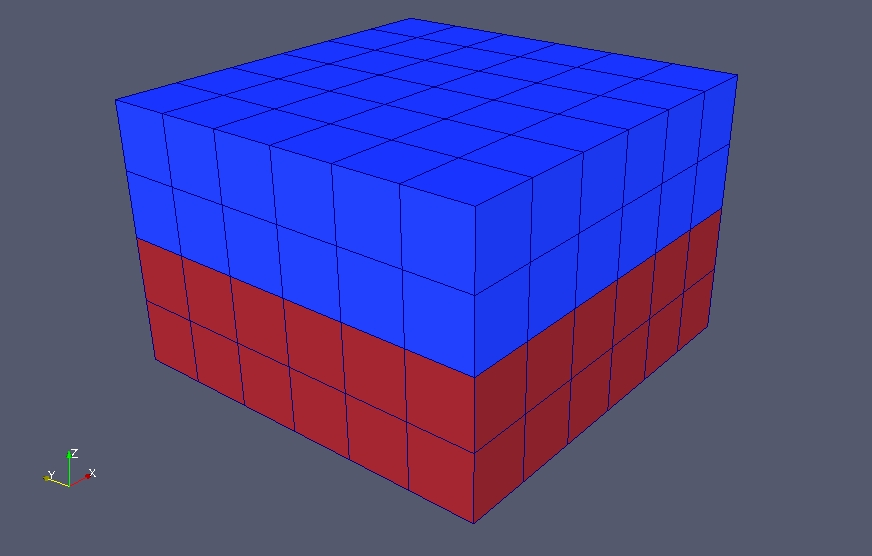
\includegraphics[scale=0.33]{tutorials/3dhex8/figs/hex8-mesh}
\par\end{centering}

\caption{Mesh composed of trilinear hexahedral cells generated by CUBIT used
for the suite of example problems. The different colors represent
the two different materials.\label{fig:3dhex8-mesh}}
\end{figure}

\par\end{center}


\subsection{Additional Common Information}

In addition to the mesh, the example problems share other information.
As in previous examples, we place this information in \texttt{pylithapp.cfg}.
Since these examples use a mesh from CUBIT, in this file we set the
importer to \texttt{MeshIOCubit}:
\begin{lyxcode}
{[}pylithapp.mesh\_generator{]}

reader~=~pylith.meshio.MeshIOCubit~\\
~\\


{[}pylithapp.mesh\_generator.reader{]}

filename~=~mesh/box\_hex8\_1000m.exo
\end{lyxcode}
This example differs from some earlier examples, because we specify
two material groups:
\begin{lyxcode}
{[}pylithapp.timedependent{]}

materials~=~{[}upper\_crust,lower\_crust{]}~\\
~\\


{[}pylithapp.timedependent.materials.upper\_crust{]}

label~=~Upper~crust~material

id~=~1

db.iohandler.filename~=~spatialdb/mat\_elastic.spatialdb

quadrature.cell~=~pylith.feassemble.FIATLagrange

quadrature.cell.dimension~=~3~\\
~\\


{[}pylithapp.timedependent.materials.lower\_crust{]}

label~=~Lower~crust~material

id~=~2

db.iohandler.filename~=~spatialdb/mat\_elastic.spatialdb

quadrature.cell~=~pylith.feassemble.FIATLagrange

quadrature.cell.dimension~=~3
\end{lyxcode}
The two material groups correspond to the two different colored regions
in Figure \vref{fig:3dhex8-mesh}. Using two material groups allows
us to specify different material types or material variations for
the upper crust and lower crust, if desired. For now, we retain the
default \texttt{ElasticIsotropic3D} material type for both materials.
This behavior will be overridden by example-specific\texttt{.cfg}
files in some of the examples. Although the material groups are specified
in \texttt{pylithapp.cfg}, the physical properties for the material
models are given in \texttt{spatialdb/}~\linebreak{}
\texttt{mat\_elastic.spatialdb}. This spatial database provides values
at a single point, resulting in uniform properties within the material.


\subsection{Example Problems}

The example problems are divided into categories that roughly correspond
to simple static problems, quasi-static problems, problems involving
fault friction, and problems where gravity is used. For the most part,
each successive example involves just adding or changing a few parameters
from the previous example. For this reason, it is advisable to go
through each example in order, starting with the simplest (static
problems).


\subsection{\label{sec:Tutorial-3d-hex8-static}Static Examples}

PyLith features discussed in this tutorial:
\begin{itemize}
\item Static solution
\item VTK output
\item Dirichlet displacement boundary conditions
\item Neumann traction boundary conditions
\item ZeroDispDB spatial database
\item SimpleDB spatial database
\item UniformDB spatial database
\item Static fault rupture
\item Specifying more than one material
\item Linearly elastic isotropic material
\end{itemize}

\subsubsection{Overview}

This set of examples describe the simplest class of problems for PyLith.
The problems are all purely elastic, and there is no time-dependence.
This set of elastostatic examples primarily demonstrates the application
of different types of boundary conditions in PyLith, as well as demonstrating
the use of a kinematic fault for a static problem. All of the examples
are contained in the directory \texttt{examples/3d/hex8}, and the
corresponding \texttt{.cfg} files are \texttt{step01.cfg}, \texttt{step02.cfg},
and \texttt{step03.cfg}. Each example may be run as follows:
\begin{lyxcode}
pylith~stepXX.cfg
\end{lyxcode}
This will cause PyLith to read the default parameters in \texttt{pylithapp.cfg},
and then override or augment them with the additional parameters in
the \texttt{stepXX.cfg} file. Each \texttt{.cfg} file is extensively
documented to provide detailed information on the various parameters.


\subsubsection{Step01 - Pure Dirichlet Boundary Conditions}

The \texttt{step01.cfg} file defines a problem with pure Dirichlet
(displacement) boundary conditions corresponding to compression in
the x-direction and shear in the y-direction. The bottom (minimum
z) boundary is held fixed in the z-direction. On the positive and
negative x-faces, compressional displacements of 1 m are applied in
the x-direction and shear displacements yielding a left-lateral sense
of shear are applied in the y-direction. In this example and in subsequent
examples we would like to output the displacement solution over a
subset of the domain corresponding to the ground surface. To do this,
we first set the output to an array of two output managers as follows:
\begin{lyxcode}
{[}pylithapp.timedependent.implicit{]}

\#~Set~the~output~to~an~array~of~2~output~managers.

\#~We~will~output~the~solution~over~the~domain~and~the~ground~surface.

output~=~{[}domain,subdomain{]}
\end{lyxcode}
We then define the subdomain output manager to correspond to a subset
of the domain:
\begin{lyxcode}
\#~Set~subdomain~component~to~OutputSolnSubset~(boundary~of~the~domain).

output.subdomain~=~pylith.meshio.OutputSolnSubset
\end{lyxcode}
Later (in the output section at the end of the file), we specify the
nodeset that corresponds to the desired output:
\begin{lyxcode}
\#~Give~basename~for~VTK~domain~output~of~solution~over~ground~surface.

{[}pylithapp.problem.formulation.output.subdomain{]}

\#~Name~of~nodeset~for~ground~surface.

label~=~face\_zpos

writer.filename~=~output/step01-groundsurf.vtk
\end{lyxcode}
For the boundary conditions, we must describe which degrees of freedom
are being constrained (\texttt{bc\_dof}), we must provide a the label
associated with the CUBIT nodeset associated with the BC, and we must
specify the type of spatial database is being used to describe the
boundary conditions. For the x-faces, we use a \texttt{SimpleDB} to
provide the displacements on the x-faces:
\begin{lyxcode}
\#~+x~face

{[}pylithapp.timedependent.bc.x\_pos{]}

bc\_dof~=~{[}0,~1{]}

label~=~face\_xpos

db\_initial~=~spatialdata.spatialdb.SimpleDB

db\_initial.label~=~Dirichlet~BC~on~+x

db\_initial.iohandler.filename~=~spatialdb/fixeddisp\_axial\_shear.spatialdb~\\
~\\


\#~-x~face

{[}pylithapp.timedependent.bc.x\_neg{]}

bc\_dof~=~{[}0,~1{]}

label~=~face\_xneg

db\_initial~=~spatialdata.spatialdb.SimpleDB

db\_initial.label~=~Dirichlet~BC~on~-x

db\_initial.iohandler.filename~=~spatialdb/fixeddisp\_axial\_shear.spatialdb
\end{lyxcode}
For a \texttt{SimpleDB}, we must provide a filename. The default spatial
database for \texttt{db\_initial} is \texttt{ZeroDispBC}, which automatically
applies zero displacements to all vertices in the nodeset, and no
filename is required (or needed). This is what we use for the bottom
of the mesh:
\begin{lyxcode}
\#~-z~face

{[}pylithapp.timedependent.bc.z\_neg{]}

bc\_dof~=~{[}2{]}

label~=~face\_zneg

db\_initial.label~=~Dirichlet~BC~on~-z
\end{lyxcode}
When we have run the simulation, the output VTK files will be contained
in \texttt{examples/3d/hex8/output} (all with a prefix of \texttt{step01}).
Results using ParaView are shown in Figure \ref{fig:step01-displ}.

\begin{figure}
\begin{centering}
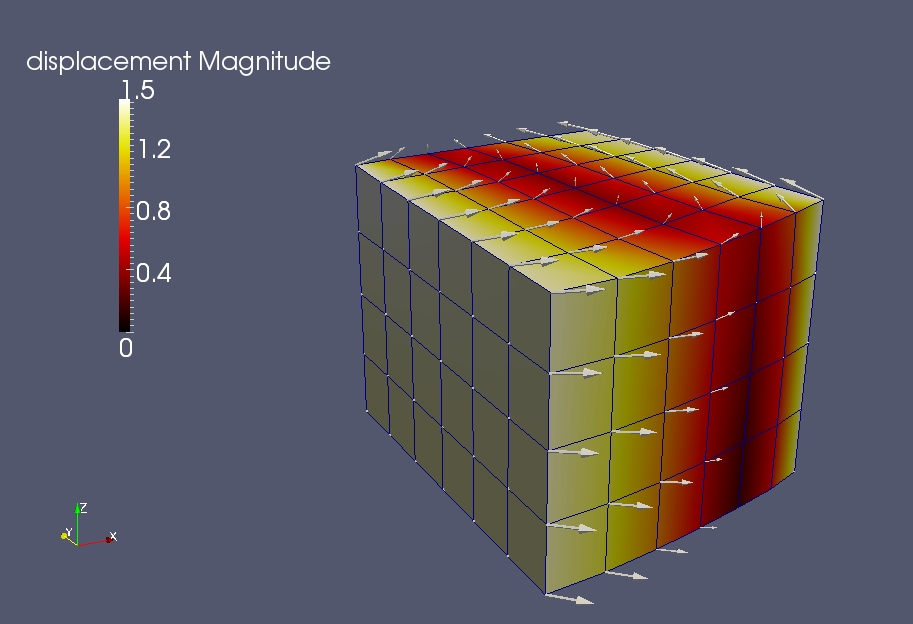
\includegraphics[width=10cm]{tutorials/3dhex8/figs/step01-displ}
\par\end{centering}

\caption{Displacement field for example step01 visualized using ParaView. The
mesh has been distorted by the computed displacements (magnified by
500), and the vectors show the computed displacements.\label{fig:step01-displ}}
\end{figure}



\subsubsection{Step02 - Dirichlet and Neumann Boundary Conditions}

The \texttt{step02.cfg} file defines a problem with Dirichlet (displacement)
boundary conditions corresponding to zero x and y-displacements applied
on the negative x-face and Neumann (traction) boundary conditions
corresponding to normal compression and horizontal shear applied on
the positive x-face. The bottom (negative z) boundary is held fixed
in the z-direction. The problem is similar to example step01, except
that 1 MPa of normal compression and 1 MPa of shear (in a left-lateral
sense) are applied on the positive x-face, and the negative x-face
is pinned in both the x and y-directions.

For the boundary conditions, we must first change the boundary condition
type for the positive x-face from the default Dirichlet to Neumann:
\begin{lyxcode}
\#~+x~face~-{}-~first~change~bc~type~to~Neumann

{[}pylithapp.timedependent.bc{]}

x\_pos~=~pylith.bc.Neumann~
\end{lyxcode}
We use a \texttt{SimpleDB} to describe the traction boundary conditions.
When applying traction boundary conditions over a surface, it is also
necessary to specify integration information for the surface. Since
this is a three-dimensional problem, the dimension of the surface
is 2. Since the cells being used are trilinear hexahedra, the cell
type is \texttt{FIATLagrange} and we use an integration order of 2.
A lower integration order would not provide sufficient accuracy while
a higher integration order would offer no benefit (while requiring
more computation time and storage):
\begin{lyxcode}
\#~+x~face

{[}pylithapp.timedependent.bc.x\_pos{]}

label~=~face\_xpos

db\_initial~=~spatialdata.spatialdb.SimpleDB

db\_initial.label~=~Neumann~BC~on~+x

db\_initial.iohandler.filename~=~spatialdb/tractions\_axial\_shear.spatialdb~\\
~\\


\#~We~must~specify~quadrature~information~for~the~cell~faces.

quadrature.cell~=~pylith.feassemble.FIATLagrange

quadrature.cell.dimension~=~2

quadrature.cell.quad\_order~=~2~
\end{lyxcode}
The boundary conditions on the negative x-face are simpler than they
were in example step01 (zero displacements in the x and y-directions),
so we can use the default \texttt{ZeroDispBC}:
\begin{lyxcode}
\#~-x~face

{[}pylithapp.timedependent.bc.x\_neg{]}

bc\_dof~=~{[}0,~1{]}~

label~=~face\_xneg

db\_initial.label~=~Dirichlet~BC~on~-x~
\end{lyxcode}
The boundary conditions on the negative z-face are supplied in the
same manner as for example step01. When we have run the simulation,
the output VTK files will be contained in \texttt{examples/3d/hex8/output}
(all with a prefix of \texttt{step02}). Results using ParaView are
shown in Figure \ref{fig:step02-displ}.
\begin{figure}
\centering{}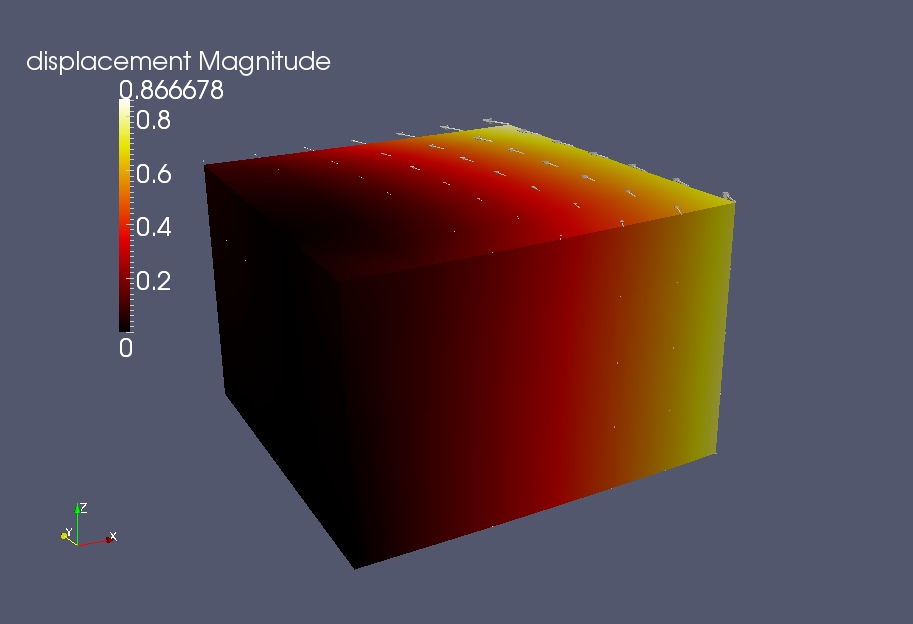
\includegraphics[width=10cm]{tutorials/3dhex8/figs/step02-displ}\caption{Displacement field for example step02 visualized using ParaView. The
mesh has been distorted by the computed displacements (magnified by
500), and the vectors show the computed displacements.\label{fig:step02-displ}.}
\end{figure}



\subsubsection{Step03 - Dirichlet Boundary Conditions with Kinematic Fault Slip}

The \texttt{step03.cfg} file describes a problem with Dirichlet (displacement)
boundary conditions corresponding to zero x and y-displacements applied
on the negative and positive x-faces and a vertical fault with a combination
of left-lateral and updip motion. The left-lateral component of fault
slip has a constant value of 2 m in the upper crust, and then decreases
linearly to zero at the base of the model. The reverse slip component
has a value of 0.25 m at the surface, and then decreases linearly
to zero at 2 km depth.

Due to the simplicity of the boundary conditions, we are able to use
the default \texttt{ZeroDispBC} for the positive and negative x-faces,
as well as the negative z-face. To use a fault, we must first define
a fault interface. We do this by providing an array containing a single
interface:
\begin{lyxcode}
{[}pylithapp.timedependent{]}

\#~Set~interfaces~to~an~array~of~1~fault:~'fault'.

interfaces~=~{[}fault{]}~
\end{lyxcode}
For this example we specify the fault slip, so we set the interface
type to \texttt{FaultCohesiveKin}:
\begin{lyxcode}
\#~Set~the~type~of~fault~interface~condition.

{[}pylithapp.timedependent.interfaces{]}

fault~=~pylith.faults.FaultCohesiveKin~
\end{lyxcode}
We must then identify the nodeset corresponding to the fault, and
provide integration information for the fault surface:
\begin{lyxcode}
\#~Set~the~parameters~for~the~fault~interface~condition.

{[}pylithapp.timedependent.interfaces.fault{]}

\#~The~label~corresponds~to~the~name~of~the~nodeset~in~CUBIT.

label~=~fault~\\
~\\


\#~We~must~define~the~quadrature~information~for~fault~cells.

\#~The~fault~cells~are~2D~(surface).

quadrature.cell~=~pylith.feassemble.FIATLagrange

quadrature.cell.dimension~=~2~
\end{lyxcode}
We retain the default \texttt{StepSlipFn} since we want static fault
slip. Finally, we use one \texttt{SimpleDB} to define the spatial
variation of fault slip, and another \texttt{SimpleDB} to define the
spatial variation in slip initiation times (the start time is 0.0
everywhere since this is a static problem):
\begin{lyxcode}
\#~The~slip~time~and~final~slip~are~defined~in~spatial~databases.~\\
{[}pylithapp.timedependent.interfaces.fault.eq\_srcs.rupture.slip\_function{]}~\\
slip.iohandler.filename~=~spatialdb/finalslip.spatialdb

slip.query\_type~=~linear

slip\_time.iohandler.filename~=~spatialdb/sliptime.spatialdb~
\end{lyxcode}
Since the problem now contains a fault, we can request that fault
infomation is also output:
\begin{lyxcode}
\#~Give~basename~for~VTK~fault~output.

{[}pylithapp.problem.interfaces.fault.output{]}

writer.filename~=~output/step03-fault.vtk~
\end{lyxcode}
This will result in two extra files being produced. The first file
(\texttt{step03-fault\_info.vtk}) contains information such as the
normal directions to the fault surface, the applied fault slip, and
the fault slip times. The second file (\texttt{step03-fault\_t0000000.vtk})
contains the cumulative fault slip for the time step and the change
in tractions on the fault surface due to the slip. When we have run
the simulation, the output VTK files will be contained in \texttt{examples/3d/hex8/output}
(all with a prefix of \texttt{step03}). Results using ParaView are
shown in Figure \ref{fig:step03-displ}.
\begin{figure}
\centering{}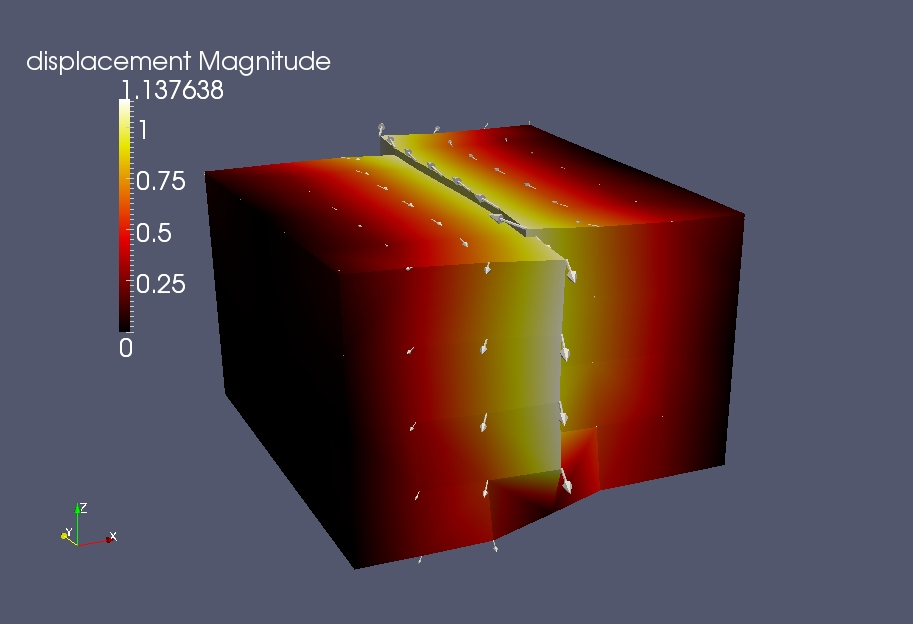
\includegraphics[width=10cm]{tutorials/3dhex8/figs/step03-displ}\caption{Displacement field for example step03 visualized using ParaView. The
mesh has been distorted by the computed displacements (magnified by
500), and the vectors show the computed displacements.\label{fig:step03-displ}.}
\end{figure}


\subsection{\label{sec:Tutorial-3d-hex8-quasistatic}Quasi-Static Examples}

PyLith features discussed in this tutorial:
\begin{itemize}
\item Quasi-static solution
\item Formatting timestamps of VTK output files
\item HDF5 output
\item Output of velocity field
\item Dirichlet displacement and velocity boundary conditions
\item Neumann traction boundary conditions and time-varying tractions
\item UniformDB spatial database
\item CompositeDB spatial database
\item Quasi-static fault rupture and fault creep
\item Multiple kinematic fault ruptures
\item Specifying more than one material
\item Nonlinear solver
\item Maxwell linear viscoelastic material
\item Power-law viscoelastic material
\item Drucker-Prager elastoplastic material
\item Adaptive time stepping
\end{itemize}

\subsubsection{Overview}

This set of examples describes a set of quasi-static problems for
PyLith. These quasi-static problems primarily demonstrate the usage
of time-dependent boundary conditions and fault slip, as well as different
rheologies. Some of the examples also demonstrate the usage of the
nonlinear solver, which is required by the nonlinear rheologies (power-law
viscoelastic and Drucker-Prager elastoplastic). Some of the examples
also demonstrate the usage of HDF5 output, which is an alternative
to the default VTK output. All of the examples are contained in the
directory \texttt{examples/3d/hex8}, and the corresponding \texttt{.cfg}
files are \texttt{step04.cfg}, \texttt{step05.cfg}, \texttt{step06.cfg},
\texttt{step07.cfg}, \texttt{step08.cfg}, and \texttt{step09.cfg}.
Each example may be run as follows:
\begin{lyxcode}
pylith~stepXX.cfg
\end{lyxcode}
This will cause PyLith to read the default parameters in \texttt{pylithapp.cfg},
and then override or augment them with the additional parameters in
the \texttt{stepXX.cfg} file. Each \texttt{.cfg} file is extensively
documented, to provide detailed information on the various parameters.


\subsubsection{Step04 - Pure Dirichlet Velocity Boundary Conditions}

The \texttt{step04.cfg} file defines a problem with x-displacements
fixed at zero on the positive and negative x-faces while velocity
boundary conditions are applied in the y-directions on the same faces,
yielding a left-lateral sense of movement. The bottom (negative z)
boundary is held fixed in the z-direction. We also use a Maxwell viscoelastic
material for the lower crust, and the simulation is run for 200 years
using a constant time-step size of 20 years. The default time stepping
behavior is \texttt{TimeStepUniform}. We retain that behavior for
this problem and provide the total simulation time and the time-step
size:
\begin{lyxcode}
\#~Change~the~total~simulation~time~to~200~years,~and~use~a~constant~time

\#~step~size~of~20~years.

{[}pylithapp.timedependent.implicit.time\_step{]}

total\_time~=~200.0{*}year

dt~=~20.0{*}year~
\end{lyxcode}
We then change the material type of the lower crust, provide a spatial
database from which to obtain the material properties (using the default
\texttt{SimpleDB}), and request additional output information for
the material:
\begin{lyxcode}
\#~Change~material~type~of~lower~crust~to~Maxwell~viscoelastic.

{[}pylithapp.timedependent{]}

materials.lower\_crust~=~pylith.materials.MaxwellIsotropic3D~\\
~\\


\#~Provide~a~spatial~database~from~which~to~obtain~property~values.

\#~Since~there~are~additional~properties~and~state~variables~for~the~Maxwell

\#~model,~we~explicitly~request~that~they~be~output.~Properties~are~named~in

\#~cell\_info\_fields~and~state~variables~are~named~in~cell\_data\_fields.

{[}pylithapp.timedependent.materials.lower\_crust{]}

db\_properties.iohandler.filename~=~spatialdb/mat\_maxwell.spatialdb

output.cell\_info\_fields~=~{[}density,mu,lambda,maxwell\_time{]}

output.cell\_data\_fields~=~{[}total\_strain,stress,viscous\_strain{]}
\end{lyxcode}
Note that the default \texttt{output.cell\_info\_fields} are those
corresponding to an elastic material (\texttt{density}, \texttt{mu},
\texttt{lambda}), and the default \texttt{output.cell\_data\_fields}
are \texttt{total\_strain} and \texttt{stress}. For materials other
than elastic, there are generally additional material properties and
state variables, and the appropriate additional fields must be specifically
requested for each material type.

This example has no displacements in the elastic solution (t = 0),
so we retain the default \texttt{ZeroDispDB} for all instances of
\texttt{db\_initial}. To apply the velocity boundary conditions, we
must specify \texttt{db\_rate}, which is zero by default. We use a
\texttt{UniformDB} to assign the velocities:
\begin{lyxcode}
\#~+x~face

{[}pylithapp.timedependent.bc.x\_pos{]}

bc\_dof~=~{[}0,~1{]}

label~=~face\_xpos

db\_initial.label~=~Dirichlet~BC~on~+x

db\_rate~=~spatialdata.spatialdb.UniformDB

db\_rate.label~=~Dirichlet~rate~BC~on~+x

db\_rate.values~=~{[}displacement-rate-x,displacement-rate-y,rate-start-time{]}

db\_rate.data~=~{[}0.0{*}cm/year,1.0{*}cm/year,0.0{*}year{]}~\\
~\\


\#~-x~face

{[}pylithapp.timedependent.bc.x\_neg{]}

bc\_dof~=~{[}0,~1{]}

label~=~face\_xneg

db\_initial.label~=~Dirichlet~BC~on~-x

db\_rate~=~spatialdata.spatialdb.UniformDB

db\_rate.label~=~Dirichlet~rate~BC~on~+x

db\_rate.values~=~{[}displacement-rate-x,displacement-rate-y,rate-start-time{]}

db\_rate.data~=~{[}0.0{*}cm/year,-1.0{*}cm/year,0.0{*}year{]}
\end{lyxcode}
Note that \texttt{db\_rate} requires a start time, which allows the
condition to be applied at any time during the simulation. For this
example, we start the velocity boundary conditions at t = 0.

Finally, we must provide information on VTK output. This is slightly
more complicated than the static case, because we must decide the
frequency with which output occurs for each output manager. We also
assign a more user-friendly format to the output file time stamp,
and we request that the time stamp is in units of 1 year (rather than
the default value of seconds):
\begin{lyxcode}
\#~Give~basename~for~VTK~domain~output~of~solution~over~domain.

{[}pylithapp.problem.formulation.output.domain{]}

\#~We~specify~that~output~occurs~in~terms~of~a~given~time~frequency,~and

\#~ask~for~output~every~40~years.~The~time~stamps~of~the~output~files~are

\#~in~years~(rather~than~the~default~of~seconds),~and~we~give~a~format~for

\#~the~time~stamp.

output\_freq~=~time\_step

time\_step~=~40.0{*}year

writer.filename~=~output/step04.vtk

writer.time\_format~=~\%04.0f

writer.time\_constant~=~1.0{*}year~\\
~\\


\#~Give~basename~for~VTK~domain~output~of~solution~over~ground~surface.

{[}pylithapp.problem.formulation.output.subdomain{]}

\#~Name~of~nodeset~for~ground~surface.

label~=~face\_zpos

\#~We~keep~the~default~output~frequency~behavior~(skip~every~n~steps),~and

\#~ask~to~skip~0~steps~between~output,~so~that~we~get~output~every~time~step.

skip~=~0

writer.filename~=~output/step04-groundsurf.vtk

writer.time\_format~=~\%04.0f

writer.time\_constant~=~1.0{*}year
\end{lyxcode}
We provide similar output information for the two materials (\texttt{upper\_crust}
and \texttt{lower\_crust}). Note that for the domain output, we requested
output in terms of a given time frequency, while for the subdomain
we requested output in terms of number of time steps. When we have
run the simulation, the output VTK files will be contained in \texttt{examples/3d/hex8/output}
(all with a prefix of \texttt{step04}). Results using ParaView are
shown in Figure \ref{fig:step04-displ-t200}.

\begin{figure}
\begin{centering}
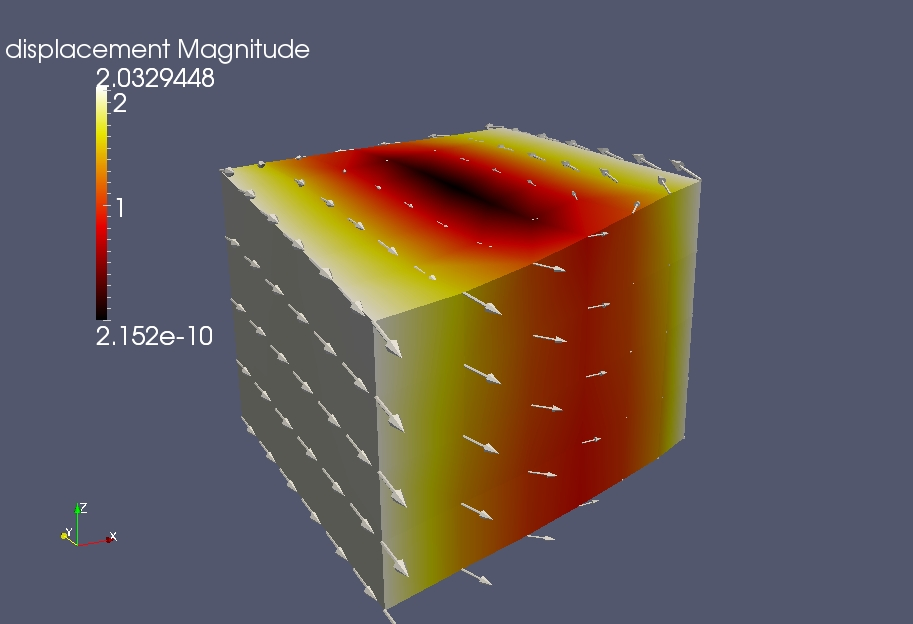
\includegraphics[width=10cm]{tutorials/3dhex8/figs/step04-displ-t200}
\par\end{centering}

\caption{Displacement field for example step04 at t = 200 years visualized
using ParaView. The mesh has been distorted by the computed displacements
(magnified by 500), and the vectors show the computed displacements.\label{fig:step04-displ-t200}}
\end{figure}



\subsubsection{Step05 - Time-Varying Dirichlet and Neumann Boundary Conditions}

The \texttt{step05.cfg} file describes a problem with time-varying
Dirichlet and Neumann boundary conditions. The example is similar
to example step04, with a few important differences:
\begin{itemize}
\item The Dirichlet boundary conditions on the negative x-face include an
initial displacement (applied in the elastic solution), as well as
a constant velocity.
\item Neumann (traction) boundary conditions are applied in the negative
x-direction on the positive x-face, giving a compressive stress. An
initial traction is applied in the elastic solution, and then at t
= 100 years it begins decreasing linearly until it reaches zero at
the end of the simulation (t = 200 years).
\end{itemize}
We again use a Maxwell viscoelastic material for the lower crust.

For the boundary conditions, we must first change the boundary condition
type for the positive x-face from the default Dirichlet to Neumann:
\begin{lyxcode}
\#~+x~face~-{}-~first~change~bc~type~to~Neumann

{[}pylithapp.timedependent.bc{]}

x\_pos~=~pylith.bc.Neumann~
\end{lyxcode}
We provide quadrature information for this face as we did for example
step02. We then use a \texttt{UniformDB} for both the initial tractions
as well as the traction rates. We provide a start time of 100 years
for the traction rates, and use a rate of 0.01 MPa/year, so that by
the end of 200 years we have completely cancelled the initial traction
of -1 MPa:
\begin{lyxcode}
{[}pylithapp.timedependent.bc.x\_pos{]}

\#~First~specify~a~UniformDB~for~the~initial~tractions,~along~with~the~values.

db\_initial~=~spatialdata.spatialdb.UniformDB

db\_initial.label~=~Neumann~BC~on~+x

db\_initial.values~=~{[}traction-shear-horiz,traction-shear-vert,traction-normal{]}

db\_initial.data~=~{[}0.0{*}MPa,0.0{*}MPa,-1.0{*}MPa{]}~\\
~\\


\#~Provide~information~on~traction~rates.

db\_rate~=~spatialdata.spatialdb.UniformDB

db\_rate.label~=~Neumann~rate~BC~on~+x

db\_rate.values~=~{[}traction-rate-shear-horiz,traction-rate-shear-vert,~\\
traction-rate-normal,rate-start-time{]}

db\_rate.data~=~{[}0.0{*}MPa/year,0.0{*}MPa/year,0.01{*}MPa/year,100.0{*}year{]}
\end{lyxcode}
The boundary conditions on the negative x-face are analogous, but
we are instead using Dirichlet boundary conditions, and the initial
displacement is in the same direction as the applied velocities:
\begin{lyxcode}
\#~-x~face

{[}pylithapp.timedependent.bc.x\_neg{]}

bc\_dof~=~{[}0,~1{]}

label~=~face\_xneg~\\
~\\


\#~Initial~displacements.

db\_initial~=~spatialdata.spatialdb.UniformDB

db\_initial.label~=~Dirichlet~BC~on~-x

db\_initial.values~=~{[}displacement-x,displacement-y{]}

db\_initial.data~=~{[}0.0{*}cm,-0.5{*}cm{]}~\\
~\\


\#~Velocities.

db\_rate~=~spatialdata.spatialdb.UniformDB

db\_rate.label~=~Dirichlet~rate~BC~on~-x

db\_rate.values~=~{[}displacement-rate-x,displacement-rate-y,rate-start-time{]}

db\_rate.data~=~{[}0.0{*}cm/year,-1.0{*}cm/year,0.0{*}year{]}
\end{lyxcode}
The boundary conditions on the negative z-face are supplied in the
same manner as for example step04. When we have run the simulation,
the output VTK files will be contained in \texttt{examples/3d/hex8/output}
(all with a prefix of \texttt{step05}). Results using ParaView are
shown in Figure \ref{fig:step05-displ-t40}.
\begin{figure}
\centering{}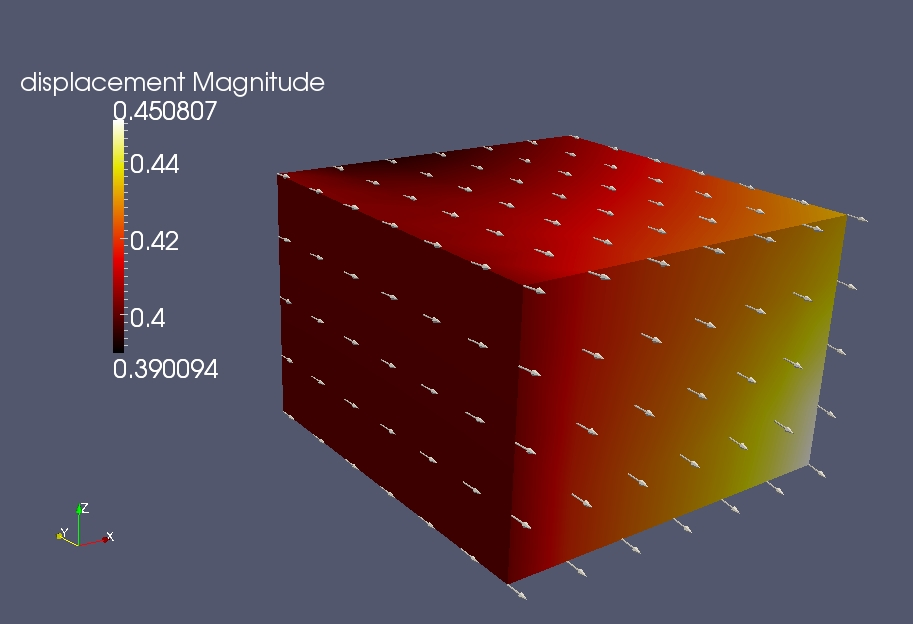
\includegraphics[width=10cm]{tutorials/3dhex8/figs/step05-displ-t40}\caption{Displacement field for example step05 at t = 40 years visualized using
ParaView. The mesh has been distorted by the computed displacements
(magnified by 500), and the vectors show the computed displacements.\label{fig:step05-displ-t40}.}
\end{figure}



\subsubsection{Step06 - Dirichlet Boundary Conditions with Time-Dependent Kinematic
Fault Slip}

The \texttt{step06.cfg} file defines a problem with Dirichlet (displacement)
boundary conditions corresponding to zero x- and y-displacements applied
on the negative and positive x-faces and a vertical fault that includes
multiple earthquake ruptures as well as steady fault creep. The upper
(locked) portion of the fault has 4 m of left-lateral slip every 200
years, while the lower (creeping) portion of the fault slips at a
steady rate of 2 cm/year. The problem bears some similarity to the
strike-slip fault model of Savage and Prescott \cite{Savage:Prescott:1978},
except that the fault creep extends through the viscoelastic portion
of the domain, and the far-field displacement boundary conditions
are held fixed.

In this example and the remainder of the examples in this section,
we change the time stepping behavior from the default \texttt{TimeStepUniform}
to \texttt{TimeStepAdapt}. For adaptive time stepping, we provide
the maximum permissible time-step size, along with a stability factor.
The stability factor controls the time-step size relative to the stable
time-step size provided by the different materials in the model. A
\texttt{stability\_factor} of 1.0 means we should use the stable time-step
size, while a \texttt{stability\_factor} greater than 1.0 means we
want to use a smaller time-step size. A \texttt{stability\_factor}
less than 1.0 allows time-step sizes greater than the stable time-step
size, which may provide inaccurate results. The adaptive time stepping
information is provided as:
\begin{lyxcode}
\#~Change~time~stepping~algorithm~from~uniform~time~step,~to~adaptive

\#~time~stepping.

time\_step~=~pylith.problems.TimeStepAdapt~\\
~\\


\#~Change~the~total~simulation~time~to~700~years,~and~set~the~maximum~time

\#~step~size~to~10~years.

{[}pylithapp.timedependent.implicit.time\_step{]}

total\_time~=~700.0{*}year

max\_dt~=~10.0{*}year

stability\_factor~=~1.0~;~use~time~step~equal~to~stable~value~from~materials
\end{lyxcode}
In this example and the remainder of the examples in this section,
we also make use of HDF5 output rather than the default VTK output.
HDF5 output is a new feature beginning with PyLith version 1.6, and
it is much more efficient with the additional advantage that multiple
time steps can be contained in a single file. PyLith also produces
Xdmf files describing the contents of the HDF5 files, which allows
the files to be read easily by applications such as ParaView. Since
VTK output is still the default, we must change the value from the
default. Also note that the filename suffix is \texttt{.h5}:
\begin{lyxcode}
\#~Give~basename~for~output~of~solution~over~domain.

{[}pylithapp.problem.formulation.output.domain{]}

\#~We~specify~that~output~occurs~in~terms~of~a~given~time~frequency,~and

\#~ask~for~output~every~50~years.

output\_freq~=~time\_step

time\_step~=~50.0{*}year~\\
~\\


\#~We~are~using~HDF5~output~so~we~must~change~the~default~writer.

writer~=~pylith.meshio.DataWriterHDF5

writer.filename~=~output/step06.h5~~
\end{lyxcode}
Note that we no longer need the \texttt{writer.time\_format} or \texttt{writer.time\_constant}
properties, since all time steps are contained in a single file. The
HDF5 writer does not have these properties, so if we attempt to define
them an error will result.

We also set the writer for other output as well, since it is not the
default. For subdomain output we use:
\begin{lyxcode}
\#~Give~basename~for~output~of~solution~over~ground~surface.

{[}pylithapp.problem.formulation.output.subdomain{]}

\#~Name~of~nodeset~for~ground~surface.

label~=~face\_zpos~\\
~\\


\#~We~keep~the~default~output~frequency~behavior~(skip~every~n~steps),~and

\#~ask~to~skip~0~steps~between~output,~so~that~we~get~output~every~time~step.

\#~We~again~switch~the~writer~to~produce~HDF5~output.

skip~=~0

writer~=~pylith.meshio.DataWriterHDF5

writer.filename~=~output/step06-groundsurf.h5~~
\end{lyxcode}
For fault output we use:
\begin{lyxcode}
\#~Give~basename~for~fault~rupture~output.

{[}pylithapp.problem.interfaces.fault.output{]}

\#~We~keep~the~default~output~frequency~behavior~(skip~every~n~steps),~and

\#~ask~to~skip~0~steps~between~output,~so~that~we~get~output~every~time~step.

\#~We~again~switch~the~writer~to~produce~HDF5~output.

skip~=~0

writer~=~pylith.meshio.DataWriterHDF5

writer.filename~=~output/step06-fault.h5
\end{lyxcode}
Due to the simplicity of the boundary conditions, we are able to use
the default \texttt{ZeroDispBC} for the positive and negative x-faces,
as well as the negative z-face. As for example step03, we define a
fault interface, we identify the nodeset corresponding to the fault,
and we provide quadrature information for the fault. We then define
an array of earthquake sources and provide an origin time for each:
\begin{lyxcode}
{[}pylithapp.timedependent.interfaces.fault{]}

\#~Set~earthquake~sources~to~an~array~consisting~of~creep~and~3~ruptures.

eq\_srcs~=~{[}creep,one,two,three{]}

eq\_srcs.creep.origin\_time~=~00.0{*}year

eq\_srcs.one.origin\_time~=~200.0{*}year

eq\_srcs.two.origin\_time~=~400.0{*}year

eq\_srcs.three.origin\_time~=~600.0{*}year
\end{lyxcode}
Note that the creep begins at t = 0 years, while the ruptures (\texttt{one},
\texttt{two}, \texttt{three}) occur at regular intervals of 200 years.
We retain the default \texttt{StepSlipFn} for the ruptures. Each of
the ruptures has the same amount of slip, and slip occurs simultaneously
for the entire rupture region, so we can use the same \texttt{SimpleDB}
files providing slip and slip time for each rupture:
\begin{lyxcode}
\#~Define~slip~and~origin~time~for~first~rupture.

{[}pylithapp.timedependent.interfaces.fault.eq\_srcs.one.slip\_function{]}

slip.iohandler.filename~=~spatialdb/finalslip\_rupture.spatialdb

slip\_time.iohandler.filename~=~spatialdb/sliptime.spatialdb~\\
~\\


\#~Define~slip~and~origin~time~for~second~rupture.

{[}pylithapp.timedependent.interfaces.fault.eq\_srcs.two.slip\_function{]}

slip.iohandler.filename~=~spatialdb/finalslip\_rupture.spatialdb

slip\_time.iohandler.filename~=~spatialdb/sliptime.spatialdb~\\
~\\


\#~Define~slip~and~origin~time~for~third~rupture.

{[}pylithapp.timedependent.interfaces.fault.eq\_srcs.three.slip\_function{]}

slip.iohandler.filename~=~spatialdb/finalslip\_rupture.spatialdb

slip\_time.iohandler.filename~=~spatialdb/sliptime.spatialdb
\end{lyxcode}
For the creep source, we change the slip function to \texttt{ConstRateSlipFn},
and we use a \texttt{SimpleDB} for both the slip time and the slip
rate:
\begin{lyxcode}
\#~Define~slip~rate~and~origin~time~for~fault~creep.

{[}pylithapp.timedependent.interfaces.fault.eq\_srcs.creep{]}

slip\_function~=~pylith.faults.ConstRateSlipFn

slip\_function.slip\_rate.iohandler.filename~=~spatialdb/sliprate\_creep.spatialdb

slip\_function.slip\_time.iohandler.filename~=~spatialdb/sliptime.spatialdb
\end{lyxcode}
For all earthquake sources we provide both an \texttt{origin\_time}
and a \texttt{slip\_function.slip\_time}. The first provides the starting
time for the entire earthquake source, while the second provides any
spatial variation in the slip time with respect to the \texttt{origin\_time}
(if any). Since there are multiple earthquake sources of different
types, there are a number of additional fault information fields available
for output. We add these additional fields' output to the fault information
file:
\begin{lyxcode}
{[}pylithapp.timedependent.interfaces.fault{]}

output.vertex\_info\_fields~=~{[}normal\_dir,strike\_dir,dip\_dir,final\_slip\_creep,~\\
final\_slip\_one,final\_slip\_two,final\_slip\_three,slip\_time\_creep,slip\_time\_one,~\\
slip\_time\_two,slip\_time\_three{]}
\end{lyxcode}
This additional information will be contained in file \texttt{step06-fault\_info.h5}.
It will contain final slip information for each earthquake source
along with slip time information. When we have run the simulation,
the output HDF5 and Xdmf files will be contained in \texttt{examples/3d/hex8/output}
(all with a prefix of \texttt{step06}). To open the files in ParaView,
the Xdmf (\texttt{.xmf}) files should be opened, as these files describe
the HDF5 data structure. Results using ParaView are shown in Figure
\ref{fig:step06-displ-t300}.
\begin{figure}
\centering{}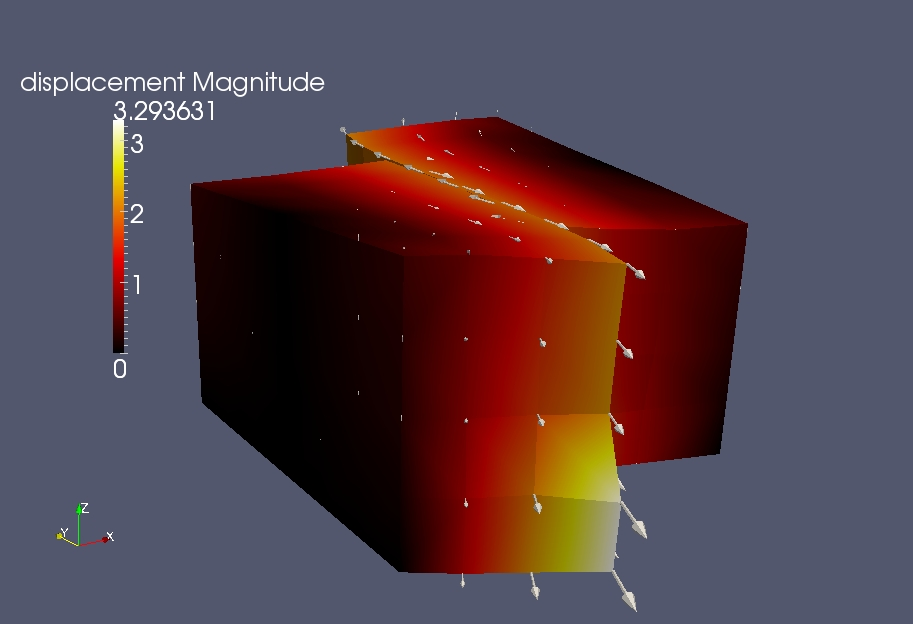
\includegraphics[width=10cm]{tutorials/3dhex8/figs/step06-displ-t300}\caption{Displacement field for example step06 at t = 300 years visualized
using ParaView. The mesh has been distorted by the computed displacements
(magnified by 500), and the vectors show the computed displacements.\label{fig:step06-displ-t300}.}
\end{figure}



\subsubsection{Step07 - Dirichlet Velocity Boundary Conditions with Time-Dependent
Kinematic Fault Slip}

In step07 we add velocity boundary conditions in the positive and
negative y-directions on the positive and negative x-faces, so that
the external boundaries keep pace with the average fault slip. This
problem is nearly identical to the strike-slip fault model of Savage
and Prescott \cite{Savage:Prescott:1978}, except that the fault creep
extends through the viscoelastic portion of the domain.

We use the default \texttt{ZeroDispBC} for the initial displacements
on the positive and negative x-faces, as well as the negative z-face.
For the velocities on the positive and negative x-faces, we use a
\texttt{UniformDB}:
\begin{lyxcode}
\#~+x~face

{[}pylithapp.timedependent.bc.x\_pos{]}

bc\_dof~=~{[}0,~1{]}

label~=~face\_xpos

db\_initial.label~=~Dirichlet~BC~on~+x

db\_rate~=~spatialdata.spatialdb.UniformDB

db\_rate.label~=~Dirichlet~rate~BC~on~+x

db\_rate.values~=~{[}displacement-rate-x,displacement-rate-y,rate-start-time{]}

db\_rate.data~=~{[}0.0{*}cm/year,1.0{*}cm/year,0.0{*}year{]}~\\
~\\


\#~-x~face

{[}pylithapp.timedependent.bc.x\_neg{]}

bc\_dof~=~{[}0,~1{]}

label~=~face\_xneg

db\_initial.label~=~Dirichlet~BC~on~-x

db\_rate~=~spatialdata.spatialdb.UniformDB

db\_rate.label~=~Dirichlet~rate~BC~on~+x

db\_rate.values~=~{[}displacement-rate-x,displacement-rate-y,rate-start-time{]}

db\_rate.data~=~{[}0.0{*}cm/year,-1.0{*}cm/year,0.0{*}year{]}
\end{lyxcode}
The fault definition information is identical to example \texttt{step06}.
In previous examples, we have just used the default output for the
domain and subdomain (ground surface), which includes the displacements.
In many cases, it is also useful to include the velocities. PyLith
provides this information, computing the velocities for the current
time step as the difference between the current displacements and
the displacements from the previous time step, divided by the time-step
size. This is more accurate than computing the velocities from the
displacement field output that has been decimated in time. We can
obtain this information by explicitly requesting it in \texttt{vertex\_data\_fields}:
\begin{lyxcode}
\#~Give~basename~for~output~of~solution~over~domain.~\\
{[}pylithapp.problem.formulation.output.domain{]}

\#~We~specify~that~output~occurs~in~terms~of~a~given~time~frequency,~and

\#~ask~for~output~every~50~years.

\#~We~also~request~velocity~output~in~addition~to~displacements.~\\
vertex\_data\_fields~=~{[}displacement,velocity{]}

output\_freq~=~time\_step

time\_step~=~50.0{*}year~\\
~\\


\#~We~are~using~HDF5~output~so~we~must~change~the~default~writer.

writer~=~pylith.meshio.DataWriterHDF5

writer.filename~=~output/step07.h5~\\
~\\


\#~Give~basename~for~output~of~solution~over~ground~surface.

{[}pylithapp.problem.formulation.output.subdomain{]}

\#~Name~of~nodeset~for~ground~surface.

label~=~face\_zpos~\\
~\\


\#~We~also~request~velocity~output~in~addition~to~displacements.

vertex\_data\_fields~=~{[}displacement,velocity{]}

\#~We~keep~the~default~output~frequency~behavior~(skip~every~n~steps),~and

\#~ask~to~skip~0~steps~between~output,~so~that~we~get~output~every~time~step.

skip~=~0~\\
~\\


\#~We~again~switch~the~writer~to~produce~HDF5~output.

writer~=~pylith.meshio.DataWriterHDF5

writer.filename~=~output/step07-groundsurf.h5
\end{lyxcode}
When we have run the simulation, the output HDF5 and Xdmf files will
be contained in \texttt{examples/3d/hex8/output} (all with a prefix
of \texttt{step07}). As for example step06, make sure to open the
\texttt{.xmf} files rather than the \texttt{.h5} files. Results using
ParaView are shown in Figure \ref{fig:step07-displ-vel-t300}.
\begin{figure}
\centering{}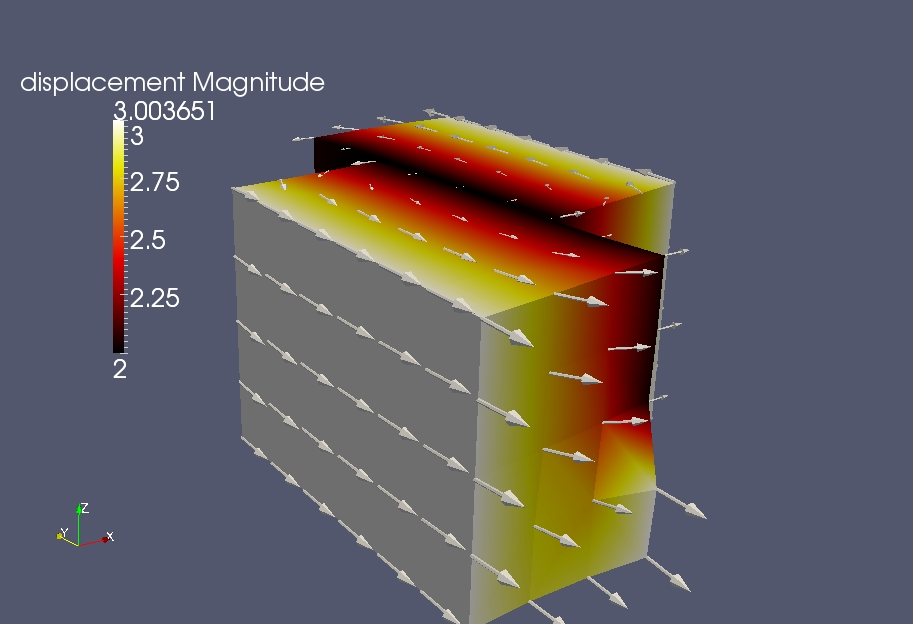
\includegraphics[width=10cm]{tutorials/3dhex8/figs/step07-displ-vel-t300}\caption{Displacement field (color contours) and velocity field (vectors) for
example step07 at t = 300 years visualized using ParaView. The mesh
has been distorted by the computed displacements (magnified by 500),
and the vectors show the computed velocities.\label{fig:step07-displ-vel-t300}}
\end{figure}



\subsubsection{Step08 - Dirichlet Velocity Boundary Conditions with Time-Dependent
Kinematic Fault Slip and Power-Law Rheology\label{sub:Tutorial-Step08-Power-law}}

The \texttt{step08.cfg} file defines a problem that is identical to
example step07, except the the lower crust is composed of a power-law
viscoelastic material. Since the material behavior is now nonlinear,
we must use the nonlinear solver:
\begin{lyxcode}
{[}pylithapp.timedependent{]}

\#~For~this~problem~we~must~switch~to~a~nonlinear~solver.

implicit.solver~=~pylith.problems.SolverNonlinear
\end{lyxcode}
Although we have not discussed the PyLith PETSc settings previously,
note that the use of the nonlinear solver may require additional options
if we wish to override the defaults. These settings are contained
in \texttt{pylithapp.cfg}:
\begin{lyxcode}
{[}pylithapp.petsc{]}

\#~Nonlinear~solver~monitoring~options.

snes\_rtol~=~1.0e-8

snes\_atol~=~1.0e-12

snes\_max\_it~=~100

snes\_monitor~=~true

snes\_view~=~true

snes\_converged\_reason~=~true
\end{lyxcode}
These settings are ignored unless we are using the nonlinear solver.

When setting the physical properties for the power-law material in
PyLith, the parameters (see Section \ref{sub:Power-Law-Maxwell-Viscoelastic})
do not generally correspond to the values provided in laboratory results.
PyLith includes a utility code, \texttt{powerlaw\_gendb.py}, to simplify
the process of using laboratory results with PyLith. This utility
code is installed in the same location as PyLith. An example of how
to use it is in \texttt{examples/3d/hex8/spatialdb/powerlaw}. The
user must provide a spatial database defining the spatial distribution
of laboratory-derived parameters (contained in \texttt{powerlaw\_params.}~\linebreak{}
\texttt{spatialdb}), another spatial database defining the temperature
field in degrees K (contained in \texttt{temperature.spatialdb}),
and a set of points for which values are desired (\texttt{powerlaw\_points.txt}).
The parameters for the code are defined in \texttt{powerlaw\_gendb.cfg}.
The properties expected by PyLith are \texttt{reference\_strain\_rate},
\texttt{reference\_stress}, and \texttt{power\_law\_exponent}. The
user must specify either \texttt{reference\_strain\_rate} or \texttt{reference\_stress}
so that \texttt{powerlaw\_gendb.py} can compute the other property.
Default values of 1.0e-6 1/s and 1 MPa are provided. In this example,
the same database was used for all parameters, and a separate database
was used to define the temperature distribution. In practice, the
user can provide any desired thermal model to provide the spatial
database for the temperature. In this example, a simple 1D (vertically-varying)
distribution was used. The utility code can be used by simply executing
it from the \texttt{examples/3d/hex8/spatialdb/powerlaw} directory:
\begin{lyxcode}
powerlaw\_gendb.py
\end{lyxcode}
This code will automatically read the parameters in \texttt{powerlaw\_gendb.cfg}
in creating the file\\
 \texttt{examples/3d/hex8/spatialdb/mat\_powerlaw.spatialdb}.

We first change the material type of the lower crust to \texttt{PowerLaw3D}:
\begin{lyxcode}
\#~Change~material~type~of~lower~crust~to~power-law~viscoelastic.

{[}pylithapp.timedependent{]}

materials.lower\_crust~=~pylith.materials.PowerLaw3D
\end{lyxcode}
In many cases, it is useful to obtain the material properties from
two different sources. For example, the elastic properties may come
from a seismic velocity model while the viscous properties may be
derived from a thermal model. In such a case we can use a \texttt{CompositeDB},
which allows a different spatial database to be used for a subset
of the properties. We do this as follows:
\begin{lyxcode}
\#~Provide~a~spatial~database~from~which~to~obtain~property~values.

\#~In~this~case,~we~prefer~to~obtain~the~power-law~properties~from~one

\#~database~and~the~elastic~properties~from~another~database,~so~we~use

\#~a~CompositeDB.~Each~part~of~the~CompositeDB~is~a~SimpleDB.

{[}pylithapp.timedependent.materials.lower\_crust{]}

db\_properties~=~spatialdata.spatialdb.CompositeDB

db\_properties.db\_A~=~spatialdata.spatialdb.SimpleDB

db\_properties.db\_B~=~spatialdata.spatialdb.SimpleDB
\end{lyxcode}
We must define the properties that come from each spatial database
and then provide the database parameters:
\begin{lyxcode}
{\small{}\#~Provide~the~values~to~be~obtained~from~each~database~and~the~database}{\small \par}

{\small{}\#~name.}{\small \par}

{\small{}{[}pylithapp.timedependent.materials.lower\_crust.db\_properties{]}}{\small \par}

{\small{}values\_A~=~{[}density,vs,vp{]}~~~;~Elastic~properties.}{\small \par}

{\small{}db\_A.label~=~Elastic~properties}{\small \par}

{\small{}db\_A.iohandler.filename~=~spatialdb/mat\_elastic.spatialdb}{\small \par}

{\small{}values\_B~=~{[}reference-stress,reference-strain-rate,power-law-exponent{]}~~~;~Power-law~properties.}{\small \par}

{\small{}db\_B.label~=~Power-law~properties}{\small \par}

{\small{}db\_B.iohandler.filename~=~spatialdb/mat\_powerlaw.spatialdb}{\small \par}
\end{lyxcode}
The \texttt{PowerLaw3D} material has additional properties and state
variables with respect to the default \texttt{ElasticIsotropic3D}
material, so we request that these properties be written to the \texttt{lower\_crust}
material files:
\begin{lyxcode}
\#~Since~there~are~additional~properties~and~state~variables~for~the

\#~power-law~model,~we~explicitly~request~that~they~be~output.~Properties~are

\#~named~in~cell\_info\_fields~and~state~variables~are~named~in

\#~cell\_data\_fields.

{[}pylithapp.timedependent.materials.lower\_crust{]}

output.cell\_info\_fields~=~{[}density,mu,lambda,reference\_strain\_rate,reference\_stress,~\\
power\_law\_exponent{]}

output.cell\_data\_fields~=~{[}total\_strain,stress,viscous\_strain{]}
\end{lyxcode}
When we have run the simulation, the output HDF5 and Xdmf files will
be contained in \texttt{examples/3d/hex8/output} (all with a prefix
of \texttt{step08}). Results using ParaView are shown in Figure \ref{fig:step08-strain-displ-t150}.
\begin{figure}
\centering{}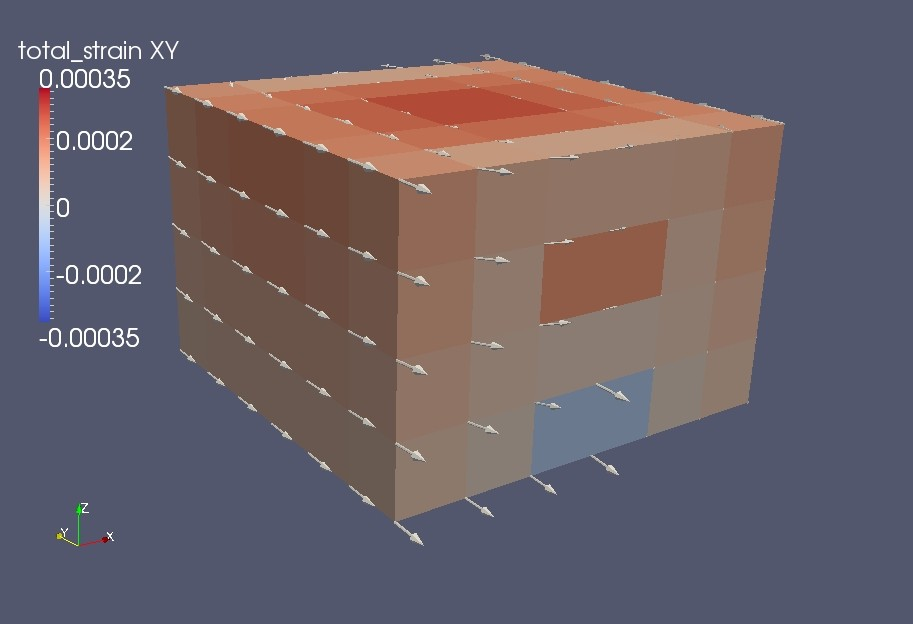
\includegraphics[width=10cm]{tutorials/3dhex8/figs/step08-strain-displ-t150}\caption{The XY-component of strain (color contours) and displacement field
(vectors) for example step08 at t = 150 years visualized using ParaView.
For this visualization, we loaded both the \texttt{step08-lower\_crust.xmf}
and \texttt{step08-upper\_crust.xmf} files to contour the strain field,
and superimposed on it the displacement field vectors from \texttt{step08.xmf}.\label{fig:step08-strain-displ-t150}}
\end{figure}



\subsubsection{Step09 - Dirichlet Velocity Boundary Conditions with Time-Dependent
Kinematic Fault Slip and Drucker-Prager Elastoplastic Rheology}

In this example we use a Drucker-Prager elastoplastic rheology in
the lower crust. As in example step08, the material behavior is nonlinear
so we again use the nonlinear solver. The material is elastoplastic,
there is no inherent time-dependent response and the stable time-step
size for the material depends on the loading conditions. To avoid
this, we set the maximum time-step size to 5 years rather than the
value of 10 years used in example \texttt{step08}:
\begin{lyxcode}
\#~Change~the~total~simulation~time~to~700~years,~and~set~the~maximum~time

\#~step~size~to~5~years.

{[}pylithapp.timedependent.implicit.time\_step{]}

total\_time~=~700.0{*}year

max\_dt~=~5.0{*}year

stability\_factor~=~1.0~;~use~time~step~equal~to~stable~value~from~materials

\#~For~this~problem~we~set~adapt\_skip~to~zero~so~that~the~time~step~size~is

\#~readjusted~every~time~step.

adapt\_skip~=~0
\end{lyxcode}
We change the material type of the lower crust to \texttt{DruckerPrager3D},
and we again use a \texttt{CompositeDB} to assign the material properties:
\begin{lyxcode}
\#~Change~material~type~of~lower~crust~to~Drucker-Prager.

{[}pylithapp.timedependent{]}

materials.lower\_crust~=~pylith.materials.DruckerPrager3D



\#~Provide~a~spatial~database~from~which~to~obtain~property~values.

\#~In~this~case,~we~prefer~to~obtain~the~Drucker-Prager~properties~from~one

\#~database~and~the~elastic~properties~from~another~database,~so~we~use

\#~a~CompositeDB.~Each~part~of~the~CompositeDB~is~a~SimpleDB.

{[}pylithapp.timedependent.materials.lower\_crust{]}

db\_properties~=~spatialdata.spatialdb.CompositeDB

db\_properties.db\_A~=~spatialdata.spatialdb.SimpleDB

db\_properties.db\_B~=~spatialdata.spatialdb.SimpleDB
\end{lyxcode}
As for the step08 example, we first define the properties that come
from each spatial database and then provide the database filename:
\begin{lyxcode}
\#~Provide~the~values~to~be~obtained~from~each~database~and~the~database

\#~name.

{[}pylithapp.timedependent.materials.lower\_crust.db\_properties{]}

values\_A~=~{[}density,vs,vp{]}~~~;~Elastic~properties.

db\_A.label~=~Elastic~properties

db\_A.iohandler.filename~=~spatialdb/mat\_elastic.spatialdb

values\_B~=~{[}friction-angle,cohesion,dilatation-angle{]}~~~;~Drucker-Prager~properties.

db\_B.label~=~Drucker-Prager~properties

db\_B.iohandler.filename~=~spatialdb/mat\_druckerprager.spatialdb
\end{lyxcode}
We also request output of the properties and state variables that
are unique to the \texttt{DruckerPrager3D} material:
\begin{lyxcode}
\#~Since~there~are~additional~properties~and~state~variables~for~the

\#~Drucker-Prager~model,~we~explicitly~request~that~they~be~output.

\#~Properties~are~named~in~cell\_info\_fields~and~state~variables~are~named~in

\#~cell\_data\_fields.

{[}pylithapp.timedependent.materials.lower\_crust{]}

output.cell\_info\_fields~=~{[}density,mu,lambda,alpha\_yield,beta,alpha\_flow{]}

output.cell\_data\_fields~=~{[}total\_strain,stress,plastic\_strain{]}
\end{lyxcode}
When we have run the simulation, the output HDF5 and Xdmf files will
be contained in \texttt{examples/3d/hex8/output} (all with a prefix
of \texttt{step09}). Results using ParaView are shown in Figure \ref{fig:step09-strain-displ-t150}.
\begin{figure}
\centering{}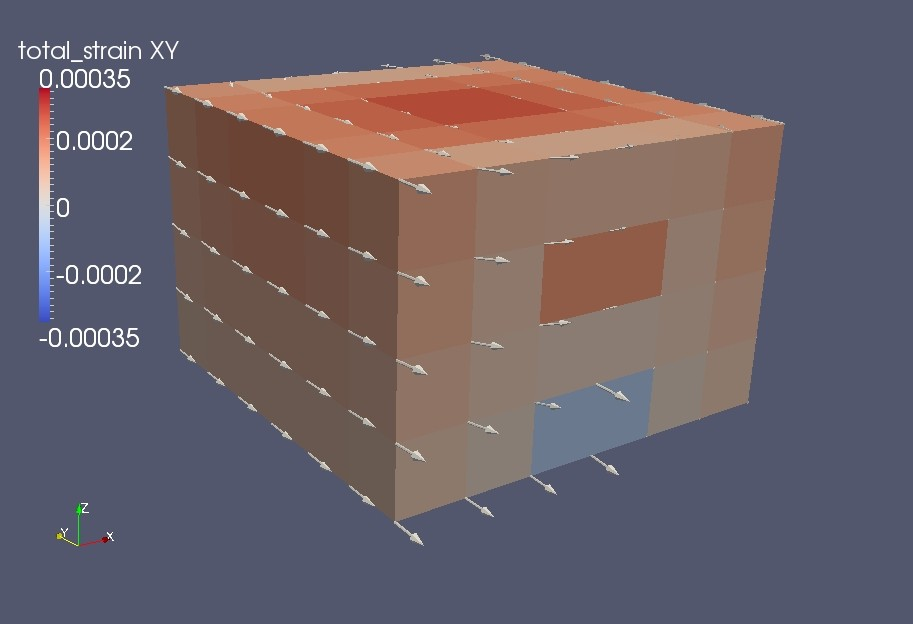
\includegraphics[width=10cm]{tutorials/3dhex8/figs/step08-strain-displ-t150}\caption{The XY-component of strain (color contours) and displacement field
(vectors) for example step09 at t = 150 years visualized using ParaView.
For this visualization, we loaded both the \texttt{step09-lower\_crust.xmf}
and \texttt{step09-upper\_crust.xmf} files to contour the strain field,
and superimposed on it the displacement field vectors from \texttt{step09.xmf}.\label{fig:step09-strain-displ-t150}}
\end{figure}


\subsection{\label{sec:Tutorial-3d-hex8-friction}Fault Friction Examples}

PyLith features discussed in this tutorial:
\begin{itemize}
\item Static fault friction
\item Slip-weakening fault friction
\item Rate-and-state fault friction
\item Nonlinear solver
\end{itemize}

\subsubsection{Overview}

This set of examples provides an introduction to using fault friction
in static and quasi-static problems with PyLith. Dynamic problems
with fault friction are discussed in Section \vref{sec:tutorial:shearwave:quad4}.
The boundary conditions are all either static or quasi-static Dirichlet
conditions, and only elastic materials are used. In all the fault
friction examples we apply axial (x) displacements on both the positive
and negative x-faces to maintain a compressive normal tractions on
the fault. Otherwise, there would be no frictional resistance. Fault
friction generates nonlinear behavior, so we use the nonlinear solver.
All of the examples are contained in the directory \texttt{examples/3d/hex8},
and the corresponding \texttt{.cfg} files are \texttt{step10.cfg},
\texttt{step11.cfg}, \texttt{step12.cfg}, \texttt{step13.cfg}, and
\texttt{step14.cfg}. Each example may be run as follows:
\begin{lyxcode}
pylith~stepXX.cfg
\end{lyxcode}
This will cause PyLith to read the default parameters in \texttt{pylithapp.cfg},
and then override or augment them with the additional parameters in
the \texttt{stepXX.cfg} file. Each \texttt{.cfg} file is extensively
documented, to provide detailed information on the various parameters.


\subsubsection{Step10 - Static Friction (Stick) with Static Dirichlet Boundary Conditions}

The \texttt{step10.cfg} file defines a problem that is identical to
example step01, except for the presence of a vertical fault with static
friction. In this case, the applied displacements are insufficient
to cause the fault to slip, so the solution is identical to that in
example step01. As in previous examples involving faults, we must
first provide an array defining the fault interfaces:
\begin{lyxcode}
{[}pylithapp.timedependent{]}

\#~Set~interfaces~to~an~array~of~1~fault:~'fault'.

interfaces~=~{[}fault{]}
\end{lyxcode}
Since all fault friction models are nonlinear we must also use the
nonlinear solver:
\begin{lyxcode}
{[}pylithapp.timedependent.implicit{]}

\#~Fault~friction~is~a~nonlinear~problem~so~we~need~to~use~the~nonlinear

\#~solver.

solver~=~pylith.problems.SolverNonlinear
\end{lyxcode}
We need to change the fault interface from the default (\texttt{FaultCohesiveKin})
to \texttt{FaultCohesiveDyn} and we set the friction model to use:
\begin{lyxcode}
{[}pylithapp.timedependent.interfaces{]}

\#~Change~fault~to~dynamic~fault~interface.

fault~=~pylith.faults.FaultCohesiveDyn~\\
~\\


{[}pylithapp.timedependent.interfaces.fault{]}

\#~Use~the~static~friction~model.

friction~=~pylith.friction.StaticFriction
\end{lyxcode}
The \texttt{StaticFriction} model requires values for the coefficient
of friction and the cohesion (see Section \vref{sec:fault:constitutive:models}).
We provide both of these using a \texttt{UniformDB}:
\begin{lyxcode}
{[}pylithapp.timedependent.interfaces.fault{]}

\#~Set~static~friction~model~parameters~using~a~uniform~DB.~Set~the

\#~static~coefficient~of~friction~to~0.6~and~cohesion~to~0.0~Pa.

friction.db\_properties~=~spatialdata.spatialdb.UniformDB

friction.db\_properties.label~=~Static~friction

friction.db\_properties.values~=~{[}friction-coefficient,cohesion{]}

friction.db\_properties.data~=~{[}0.6,0.0{*}Pa{]}
\end{lyxcode}
Fault friction models require additional PETSc settings:
\begin{lyxcode}
\#~NOTE:~There~are~additional~settings~specific~to~fault~friction.

{[}pylithapp.petsc{]}

\#~Friction~sensitivity~solve~used~to~compute~the~increment~in~slip

\#~associated~with~changes~in~the~Lagrange~multiplier~imposed~by~the

\#~fault~constitutive~model.

friction\_pc\_type~=~asm

friction\_sub\_pc\_factor\_shift\_type~=~nonzero

friction\_ksp\_max\_it~=~25

friction\_ksp\_gmres\_restart~=~30

\#~Uncomment~to~view~details~of~friction~sensitivity~solve.

\#friction\_ksp\_monitor~=~true

\#friction\_ksp\_view~=~true

friction\_ksp\_converged\_reason~=~true


\end{lyxcode}
When we have run the simulation, the output VTK files will be contained
in \texttt{examples/3d/hex8/output} (all with a pvrefix of \texttt{step10}).
Results using ParaView are shown in Figure \vref{fig:step10-fault-traction-slip}.

\begin{figure}
\begin{centering}
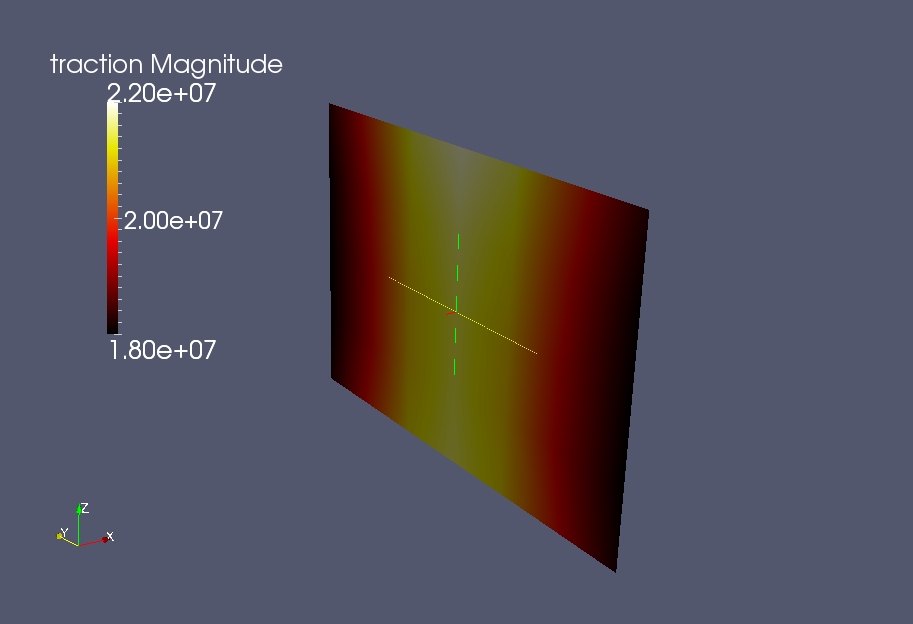
\includegraphics[width=10cm]{tutorials/3dhex8/figs/step10-fault-traction-slip}
\par\end{centering}

\caption{Magnitude of tractions on the fault for example step10 visualized
using ParaView. \label{fig:step10-fault-traction-slip}}
\end{figure}



\subsubsection{Step11 - Static Friction (Slip) with Static Dirichlet Boundary Conditions}

In step11 we apply twice as much shear displacement as in step10,
which is sufficient to induce slip on the fault. All other settings
are identical. To change the amount of shear displacement, we change
the spatial database for the positive and negative x-faces to a \texttt{UniformDB},
and apply the altered values within the \texttt{.cfg} file:
\begin{lyxcode}
\#~+x~face

{[}pylithapp.timedependent.bc.x\_pos{]}

bc\_dof~=~{[}0,~1{]}

label~=~face\_xpos

db\_initial~=~spatialdata.spatialdb.UniformDB

db\_initial.label~=~Dirichlet~BC~on~+x

db\_initial.values~=~{[}displacement-x,displacement-y{]}

db\_initial.data~=~{[}-1.0{*}m,2.0{*}m{]}



\#~-x~face

{[}pylithapp.timedependent.bc.x\_neg{]}

bc\_dof~=~{[}0,~1{]}

label~=~face\_xneg

db\_initial~=~spatialdata.spatialdb.UniformDB

db\_initial.label~=~Dirichlet~BC~on~-x

db\_initial.values~=~{[}displacement-x,displacement-y{]}

db\_initial.data~=~{[}1.0{*}m,-2.0{*}m{]}
\end{lyxcode}
When we have run the simulation, the output VTK files will be contained
in \texttt{examples/3d/hex8/output} (all with a pvrefix of \texttt{step11}).
Results using ParaView are shown in Figure \vref{fig:step11-fault-traction-slip}.

\begin{figure}
\begin{centering}
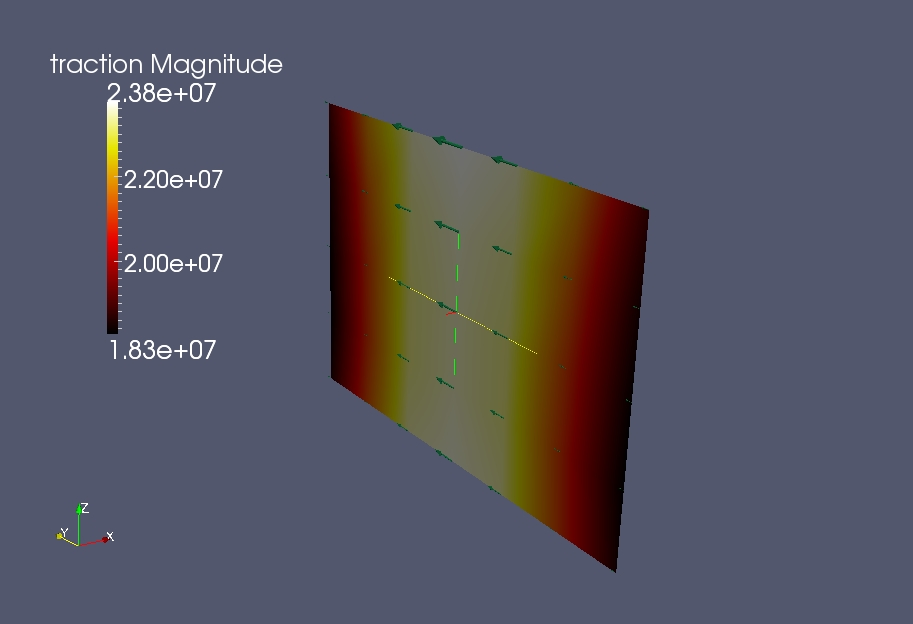
\includegraphics[width=10cm]{tutorials/3dhex8/figs/step11-fault-traction-slip}
\par\end{centering}

\caption{Magnitude of tractions on the fault for example step10 visualized
using ParaView. Vectors of fault slip are also plotted. Note that
PyLith outputs slip in the fault coordinate system, so we transform
them to the global coordinate system using the Calculator in ParaView.
A more general approach involves outputing the fault coordinate system
information and using these fields in the Calculator. \label{fig:step11-fault-traction-slip}}
\end{figure}



\subsubsection{Step12 - Static Friction with Quasi-Static Dirichlet Boundary Conditions}

The \texttt{step12.cfg} file describes a problem that is similar to
examples step10 and step11, except that we apply velocity boundary
conditions and run the simulation for 200 years. Once fault friction
is overcome, the fault slips at a steady rate. To prevent convergence
problems we set the time step size to a constant value of 5 years:
\begin{lyxcode}
\#~Change~the~total~simulation~time~to~200~years,~and~use~a~constant~time

\#~step~size~of~5~years.

{[}pylithapp.timedependent.implicit.time\_step{]}

total\_time~=~200.0{*}year

dt~=~5.0{*}year
\end{lyxcode}
As in the other fault friction examples, we apply initial displacements
along the x-axis (to maintain a compressive stress on the fault),
and we apply velocity boundary conditions that yield a left-lateral
sense of motion:
\begin{lyxcode}
\#~+x~face~-{}-~Dirichlet

{[}pylithapp.timedependent.bc.x\_pos{]}

bc\_dof~=~{[}0,1{]}

label~=~face\_xpos

db\_initial~=~spatialdata.spatialdb.UniformDB

db\_initial.label~=~Dirichlet~BC~on~+x

db\_initial.values~=~{[}displacement-x,displacement-y{]}

db\_initial.data~=~{[}-1.0{*}m,0.0{*}m{]}

db\_rate~=~spatialdata.spatialdb.UniformDB

db\_rate.label~=~Dirichlet~rate~BC~on~+x

db\_rate.values~=~{[}displacement-rate-x,displacement-rate-y,rate-start-time{]}

db\_rate.data~=~{[}0.0{*}cm/year,1.0{*}cm/year,0.0{*}year{]}~\\
~\\


\#~-x~face

{[}pylithapp.timedependent.bc.x\_neg{]}

bc\_dof~=~{[}0,~1{]}

label~=~face\_xneg

db\_initial.label~=~Dirichlet~BC~on~-x

db\_rate~=~spatialdata.spatialdb.UniformDB

db\_rate.label~=~Dirichlet~rate~BC~on~-x

db\_rate.values~=~{[}displacement-rate-x,displacement-rate-y,rate-start-time{]}

db\_rate.data~=~{[}0.0{*}cm/year,-1.0{*}cm/year,0.0{*}year{]}
\end{lyxcode}
For this example, we keep the same coefficient of friction as examples
step10 and step11, but we include a cohesion of 2 MPa:
\begin{lyxcode}
{[}pylithapp.timedependent.interfaces.fault{]}

\#~Set~static~friction~model~parameters~using~a~uniform~DB.~Set~the

\#~static~coefficient~of~friction~to~0.6~and~cohesion~to~2.0~MPa.

friction.db\_properties~=~spatialdata.spatialdb.UniformDB

friction.db\_properties.label~=~Static~friction

friction.db\_properties.values~=~{[}friction-coefficient,cohesion{]}

friction.db\_properties.data~=~{[}0.6,2.0{*}MPa{]}
\end{lyxcode}
When we have run the simulation, the output VTK files will be contained
in \texttt{examples/3d/hex8/output} (all with a pvrefix of \texttt{step12}).
Results using ParaView are shown in Figure \vref{fig:step12-displ-t200}.

\begin{figure}
\begin{centering}
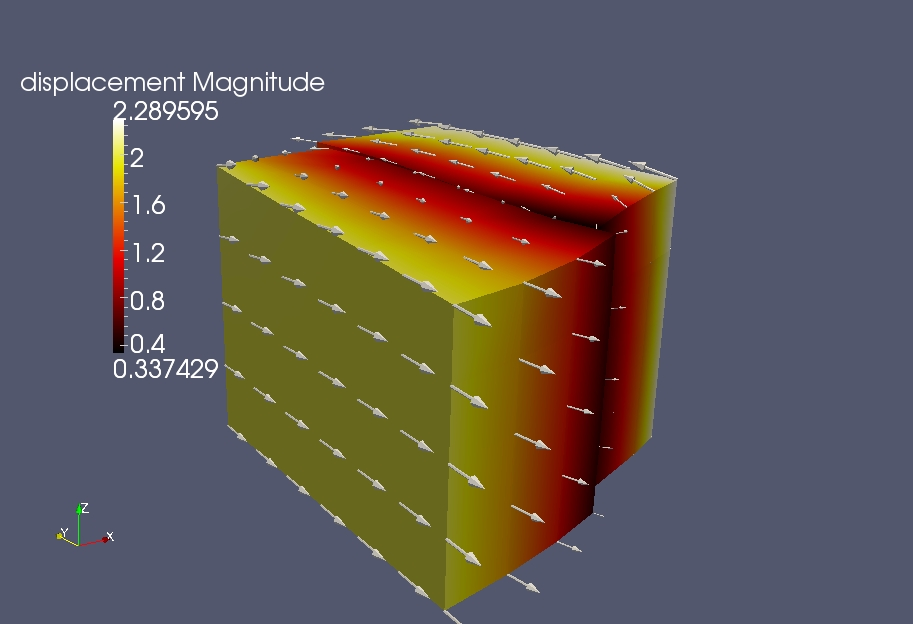
\includegraphics[width=10cm]{tutorials/3dhex8/figs/step12-displ-t200}
\par\end{centering}

\caption{Displacement field for example step12 at t = 200 years visualized
using ParaView. The mesh has been distorted by the computed displacements
(magnified by 500), and the vectors show the computed displacements.\label{fig:step12-displ-t200}}
\end{figure}



\subsubsection{Step13 - Slip-Weakening Friction with Quasi-Static Dirichlet Boundary
Conditions}

In this example we replace the static friction fault constitutive
model in step12 with a slip-weakening friction fault constitutive
model. Fault friction is overcome at about t = 80 years, the fault
slips in each subsequent time step. We again use a constant time step
size of 5 years and apply the same intial displacement and velocity
boundary conditions.

We first define the friction model for the simulation:
\begin{lyxcode}
{[}pylithapp.timedependent.interfaces.fault{]}

\#~Use~the~slip-weakening~friction~model.

friction~=~pylith.friction.SlipWeakening
\end{lyxcode}
The slip-weakening constitutive model requires a static coefficient
of friction, a dynamic coefficient of friction, a slip weakening parameter,
and a cohesion (see Section \vref{sec:fault:constitutive:models}):
\begin{lyxcode}
{[}pylithapp.timedependent.interfaces.fault{]}

\#~Set~slip-weakening~friction~model~parameters~using~a~uniform~DB.~Set~the

\#~parameters~as~follows:

\#~static~coefficient~of~friction:~0.6

\#~dynamic~coefficient~of~friction:~0.5

\#~slip-weakening~parameter:~0.2~m

\#~cohesion:~0~Pa

friction.db\_properties~=~spatialdata.spatialdb.UniformDB

friction.db\_properties.label~=~Slip~weakening

friction.db\_properties.values~=~{[}static-coefficient,dynamic-coefficient,~\\
slip-weakening-parameter,cohesion{]}

friction.db\_properties.data~=~{[}0.6,0.5,0.2{*}m,0.0{*}Pa{]}
\end{lyxcode}
When we have run the simulation, the output VTK files will be contained
in \texttt{examples/3d/hex8/output} (all with a pvrefix of \texttt{step1}3).
Results using ParaView are shown in Figure \vref{fig:step13-displ-t200}.

\begin{figure}
\begin{centering}
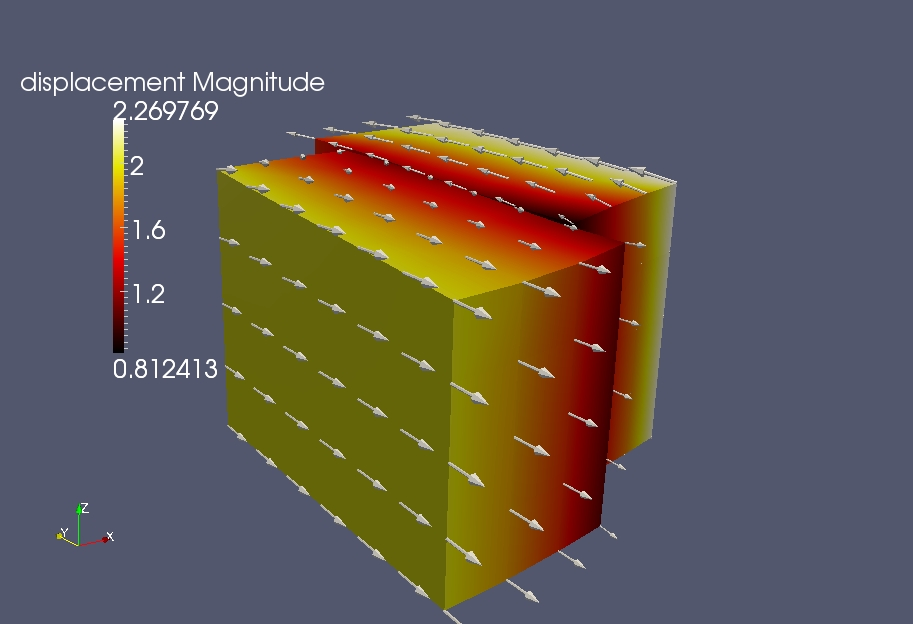
\includegraphics[width=10cm]{tutorials/3dhex8/figs/step13-displ-t200}
\par\end{centering}

\caption{Displacement field for example step13 at t = 200 years visualized
using ParaView. The mesh has been distorted by the computed displacements
(magnified by 500), and the vectors show the computed displacements.\label{fig:step13-displ-t200}}
\end{figure}



\subsubsection{Step14 - Rate-and-State Friction with Quasi-Static Dirichlet Boundary
Conditions}

In step14 we use a rate-and-state friction model with an ageing law
instead of a slip-weakening friction model. Slip begins to occur at
about t = 45 years, and continues in each subsequent time step. We
again use a constant time step size of 5 years and apply the same
intial displacement and velocity boundary conditions.

We first define the friction model for the simulation:
\begin{lyxcode}
{[}pylithapp.timedependent.interfaces.fault{]}

\#~Use~the~rate-and-state~aging~friction~model.

friction~=~pylith.friction.RateStateAgeing
\end{lyxcode}
The rate-and-state constitutive model requires a vreference coefficient
of friction, a vreference slip rate, a slip weakening parameter, an
a-value, a b-value, and a cohesion (see \vref{sec:fault:constitutive:models}):
\begin{lyxcode}
{\small{}{[}pylithapp.timedependent.interfaces.fault{]}}{\small \par}

{\small{}\#~Set~rate-and-state~parameters~using~a~UniformDB.~Set~the~parameters~as}{\small \par}

{\small{}\#~follows:}{\small \par}

{\small{}\#~vreference~coefficient~of~friction:~0.6}{\small \par}

{\small{}\#~vreference~slip~rate:~1.0e-06~m/s}{\small \par}

{\small{}\#~slip-weakening~parameter:~0.037~m}{\small \par}

{\small{}\#~a:~0.0125}{\small \par}

{\small{}\#~b:~0.0172}{\small \par}

{\small{}\#~cohesion:~0~Pa}{\small \par}

{\small{}friction.db\_properties~=~spatialdata.spatialdb.UniformDB}{\small \par}

{\small{}friction.db\_properties.label~=~Rate~State~Ageing}{\small \par}

{\small{}friction.db\_properties.values~=~{[}vreference-friction-coefficient,vreference-slip-rate,}~\\
{\small{}characteristic-slip-distance,constitutive-parameter-a,constitutive-parameter-b,cohesion{]}}{\small \par}

{\small{}friction.db\_properties.data~=~{[}0.6,1.0e-6{*}m/s,0.0370{*}m,0.0125,0.0172,0.0{*}Pa{]}}{\small \par}
\end{lyxcode}
For this model, we also want to set the initial value of the state
variable:
\begin{lyxcode}
{[}pylithapp.timedependent.interfaces.fault{]}

\#~Set~spatial~database~for~the~initial~value~of~the~state~variable.

friction.db\_initial\_state~=~spatialdata.spatialdb.UniformDB

friction.db\_initial\_state.label~=~Rate~State~Ageing~State

friction.db\_initial\_state.values~=~{[}state-variable{]}

friction.db\_initial\_state.data~=~{[}92.7{*}s{]}
\end{lyxcode}
When we have run the simulation, the output VTK files will be contained
in \texttt{examples/3d/hex8/output} (all with a pvrefix of \texttt{step14}).
Results using ParaView are shown in Figure \vref{fig:step14-displ-t200}.

\begin{figure}
\begin{centering}
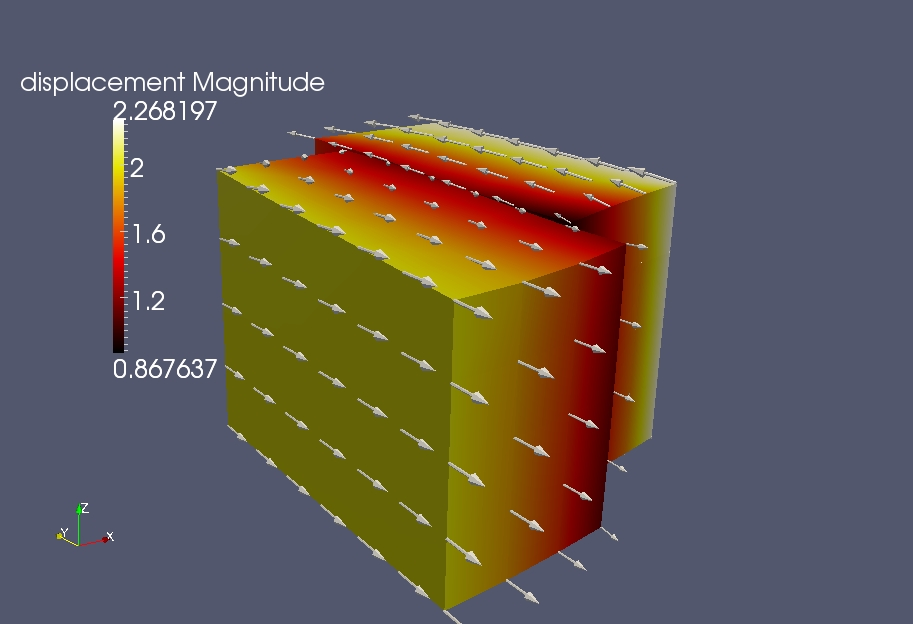
\includegraphics[width=10cm]{tutorials/3dhex8/figs/step14-displ-t200}
\par\end{centering}

\caption{Displacement field for example step14 at t = 200 years visualized
using ParaView. The mesh has been distorted by the computed displacements
(magnified by 500), and the vectors show the computed displacements.\label{fig:step14-displ-t200}}
\end{figure}


\subsection{\label{sec:Tutorial-3d-hex8-gravity}Gravitational Body Force Examples}

PyLith features discussed in this tutorial:
\begin{itemize}
\item Gravitational body forces
\item Initial stresses
\item Finite strain
\item Generalized Maxwell linear viscoelastic material
\end{itemize}

\subsubsection{Overview}

This set of examples describes a set of problems for PyLith involving
gravitational body forces. All of the examples are quasi-static and
run for a time period of 200 years. These examples also demonstrate
the use of a generalized Maxwell viscoelastic material, which is used
for the lower crust in all examples. The final example (step17) demonstrates
the usage of a finite strain formulation, which automatically invokes
the nonlinear solver. All of the examples are contained in the directory
\texttt{examples/3d/hex8}, and the corresponding \texttt{.cfg} files
are \texttt{step15.cfg}, \texttt{step16.cfg}, and \texttt{step17.cfg}.
Each example may be run as follows:
\begin{lyxcode}
pylith~stepXX.cfg
\end{lyxcode}
This will cause PyLith to read the default parameters in \texttt{pylithapp.cfg},
and then override or augment them with the additional parameters in
the \texttt{stepXX.cfg} file. Each \texttt{.cfg} file is extensively
documented, to provide detailed information on the various parameters.


\subsubsection{Step15 - Gravitational Body Forces}

The \texttt{step15.cfg} file defines a problem with extremely simple
Dirichlet boundary conditions. On the positive and negative x-faces,
the positive and negative y-faces, and the negative z-face, the displacements
normal to the face are set to zero. Because all of the materials in
the example have the same density, the elastic solution for loading
via gravitational body forces is
\begin{equation}
\sigma_{zz}=\rho gh;\:\sigma_{xx}=\sigma_{yy}=\frac{\nu\rho gh}{1-\nu}\:.\label{eq:1-1}
\end{equation}


We first set the gravity field, which by default has values of 9.80655
$\unitfrac{m}{s^{2}}$ for acceleration and $\left[0,0,-1\right]$
for direction:
\begin{lyxcode}
{[}pylithapp.timedependent{]}

\#~Set~gravity~field~(default~is~None)

gravity\_field~=~spatialdata.spatialdb.GravityField
\end{lyxcode}
We use adaptive time stepping, set the simulation time to 200 years,
and specify a maximum time step size of 10 years:
\begin{lyxcode}
{[}pylithapp.timedependent.implicit{]}

\#~Change~time~stepping~algorithm~from~uniform~time~step,~to~adaptive

\#~time~stepping.

time\_step~=~pylith.problems.TimeStepAdapt~\\
~\\


\#~Change~the~total~simulation~time~to~200~years,~and~set~the~maximum~time

\#~step~size~to~10~years.

{[}pylithapp.timedependent.implicit.time\_step{]}

total\_time~=~200.0{*}year

max\_dt~=~10.0{*}year

stability\_factor~=~1.0~;~use~time~step~equal~to~stable~value~from~materials
\end{lyxcode}
We use a generalized Maxwell model for the lower crust (see Section
\vref{sub:Formulation-for-Gen-Max}), and use a \texttt{SimpleDB} to
provide the properties. We also request the relevant properties and
state variables for output:
\begin{lyxcode}
\#~Change~material~type~of~lower~crust~to~generalized~Maxwell~viscoelastic.

{[}pylithapp.timedependent{]}

materials.lower\_crust~=~pylith.materials.GenMaxwellIsotropic3D

\#~Provide~a~spatial~database~from~which~to~obtain~property~values.

\#~Since~there~are~additional~properties~and~state~variables~for~the

\#~generalized~Maxwell~model,~we~explicitly~request~that~they~be~output.

\#~Properties~are~named~in~cell\_info\_fields~and~state~variables~are~named~in

\#~cell\_data\_fields.

{[}pylithapp.timedependent.materials.lower\_crust{]}

db\_properties.iohandler.filename~=~spatialdb/mat\_genmaxwell.spatialdb

output.cell\_info\_fields~=~{[}density,mu,lambda,shear\_ratio,maxwell\_time{]}

output.cell\_data\_fields~=~{[}total\_strain,stress,viscous\_strain\_1,viscous\_strain\_2,~\\
viscous\_strain\_3{]}
\end{lyxcode}
The boundary conditions for this example are trivial, so we are able
to use the default \texttt{ZeroDispDB} for all faces. When we have
run the simulation, the output VTK files will be contained in \texttt{examples/3d/hex8/output}
(all with a pvrefix of \texttt{step15}). Results using ParaView are
shown in Figure \vref{fig:step15-displ-t200}.

\begin{figure}
\begin{centering}
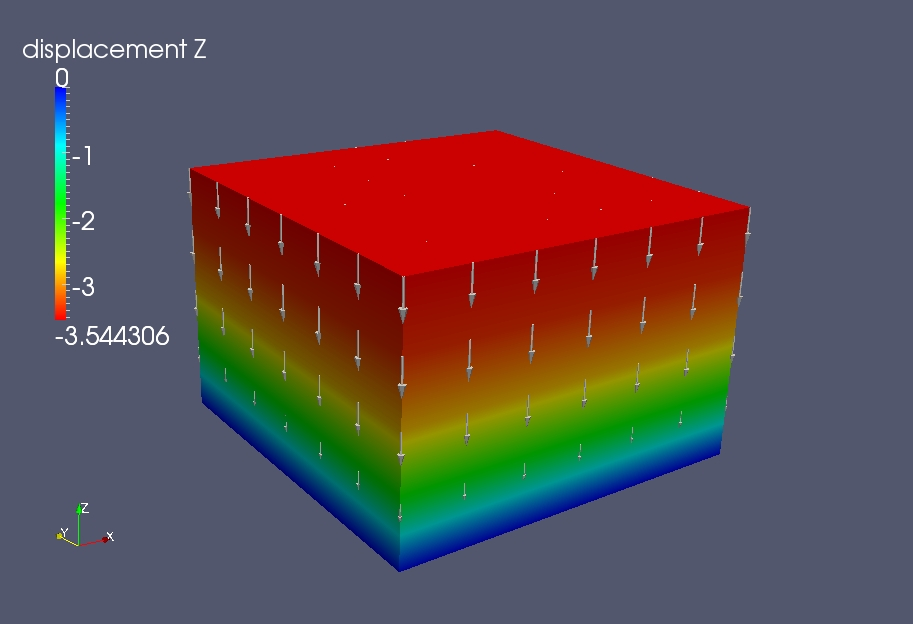
\includegraphics[width=10cm]{tutorials/3dhex8/figs/step15-displ-t200}
\par\end{centering}

\caption{Displacement field for example step15 at t = 200 years visualized
using ParaView. The z-component of the displacement field is shown
with the color contours, and the vectors show the computed displacements.\label{fig:step15-displ-t200}}


\end{figure}



\subsubsection{Step16 - Gravitational Body Forces with Initial Stresses}

The \texttt{step16.cfg} file defines a problem that is identical to
example step15, except that initial stresses are used to prevent the
initial large displacements due to 'turning on' gravity. Since all
normal stress components are given an initial stress of $\rho gh$,
the initial stress state is lithostatic, which is an appropriate condition
for many tectonic problems in the absence of tectonic stresses (e.g.,
McGarr \cite{McGarr:1988}). When compared to example step15, this
example should maintain a lithostatic state of stress for the entire
simulation, and displacements should remain essentially zero.

We set the gravity field, as in example step15, and we again use adaptive
time stepping with a generalized Maxwell rheology for the lower crust.
We provide values for the initial stress for both the upper and lower
crust. Since the materials have the same density, we are able to use
the same \texttt{SimpleDB} with a linear variation for both (see file
\texttt{examples/3d/hex8/spatialdb/initial\_stress.spatialdb}):
\begin{lyxcode}
\#~We~must~specify~initial~stresses~for~each~material.

\#~We~provide~a~filename~for~the~spatial~database~that~gives~the~stresses,

\#~and~we~change~the~query\_type~from~the~default~'nearest'~to~'linear'.

{[}pylithapp.timedependent.materials.upper\_crust{]}

db\_initial\_stress~=~spatialdata.spatialdb.SimpleDB

db\_initial\_stress.iohandler.filename~=~spatialdb/initial\_stress.spatialdb

db\_initial\_stress.query\_type~=~linear~\\
~\\


{[}pylithapp.timedependent.materials.lower\_crust{]}

db\_initial\_stress~=~spatialdata.spatialdb.SimpleDB

db\_initial\_stress.iohandler.filename~=~spatialdb/initial\_stress.spatialdb

db\_initial\_stress.query\_type~=~linear
\end{lyxcode}
Note that we use a \texttt{linear} \texttt{query\_type} rather than
the default type of \texttt{nearest}, so that a linear interpolation
is performed along the z-direction. When we have run the simulation,
the output VTK files will be contained in \texttt{examples/3d/hex8/output}
(all with a pvrefix of \texttt{step16}). Results using ParaView are
shown in Figure \vref{fig:step16-stress_xx-t200}.

\begin{figure}
\begin{centering}
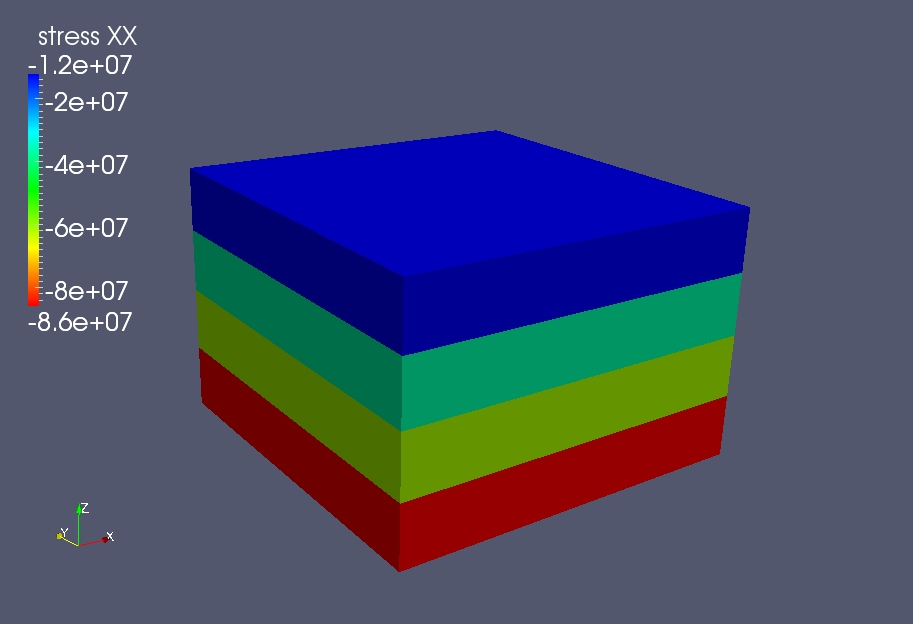
\includegraphics[width=10cm]{tutorials/3dhex8/figs/step16-stress_xx-t200}
\par\end{centering}

\caption{Stress field (xx-component) for example step16 at t = 200 years visualized
using ParaView. Note that for this example, Stress\_xx = Stress\_yy
= Stress\_zz, and there is no vertical displacement throughout the
simulation. Also note that the stresses appear as four layers since
we have used \texttt{CellFilterAvg} for material output.\label{fig:step16-stress_xx-t200}}
\end{figure}



\subsubsection{Step17 - Gravitational Body Forces with Small Strain}

The \texttt{step17.cfg} file defines a problem that is identical to
example step15, except that we now use a small strain formulation
(see Section \vref{sec:small:strain:formulation}). All of the problems
up to this point have assumed infinitesimal strain, meaning that the
change in shape of the domain during deformation is not taken into
account. In many problems it is important to consider the change in
shape of the domain. This is particularly important in many problems
involving gravitational body forces, since a change in shape of the
domain results in a different stress field. By examining the stress
and deformation fields for this example in comparison with those of
example step15, we can see what effect the infinitesimal strain approximation
has on our solution.

We set the gravity field, as in example step15 and again use adaptive
time stepping withs a generalized Maxwell rheology for the lower crust.
The only change is that we change the problem formulation from the
default \texttt{Implicit} to \texttt{ImplicitLgDeform}. Since the
large deformation formulation is nonlinear, PyLith automatically switches
the solver from the default \texttt{SolverLinear} to \texttt{SolverNonlinear}.
It is thus only necessary to change the formulation:
\begin{lyxcode}
{[}pylithapp.timedependent{]}

\#~Set~the~formulation~for~finite~strain.~The~default~solver~will

\#~automatically~be~switched~to~the~nonlinear~solver.

formulation~=~pylith.problems.ImplicitLgDeform
\end{lyxcode}
When we have run the simulation, the output VTK files will be contained
in \texttt{examples/3d/hex8/output} (all with a pvrefix of \texttt{step17}).
Results using ParaView are shown in Figure \vref{fig:step17-disp-t200}.

\begin{figure}
\begin{centering}
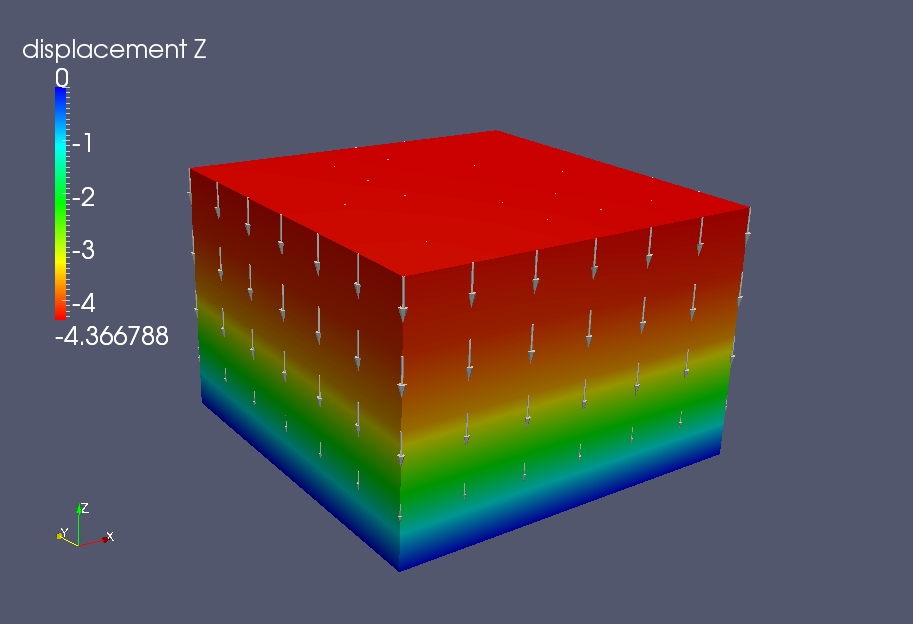
\includegraphics[width=10cm]{tutorials/3dhex8/figs/step17-displ-t200}
\par\end{centering}

\caption{Displacement field for example step17 at t = 200 years visualized
using ParaView. The z-component of the displacement field is shown
with the color contours, and the vectors show the computed displacements.
Note the larger displacements compared with example step15.\label{fig:step17-disp-t200}}
\end{figure}


\subsection{\label{sec:Tutorial-3d-hex8-surfload}Surface Load Traction Examples}

PyLith features discussed in this tutorial:
\begin{itemize}
\item Time-dependent Neumann (traction) boundary conditions
\item Dirichlet boundary conditions
\item Elastic material
\item Output of solution at user-defined locations
\end{itemize}

\subsubsection{Overview}

This set of examples describes a set of problems for PyLith involving
surface loading with a Neumann (traction) applied to the ground surface.
The first example demonstrates the use of a surface load in a static
problem, and the second example demonstates how to apply a cyclic
load in a quasi-static problem. The second problem also includes output
of the solution at user-defined locations. All of the examples are
contained in the directory \texttt{examples/3d/hex8}, and the corresponding
\texttt{.cfg} files are \texttt{step18.cfg} and \texttt{step19.cfg}.
Each example may be run as follows:
\begin{lyxcode}
pylith~stepXX.cfg
\end{lyxcode}
This will cause PyLith to read the default parameters in \texttt{pylithapp.cfg},
and then override or augment them with the additional parameters in
the \texttt{stepXX.cfg} file. Each \texttt{.cfg} file is extensively
documented, to provide detailed information on the various parameters.


\subsubsection{Step18 - Static Surface Load}

The \texttt{step18.cfg} file defines a problem with a spatially varying
axial surface load applied to the top surface with Dirichlet (roller)
boundary conditions on the lateral and bottom surfaces. We first set
the array of boundary conditions with one for each surface of the
domain. As in the other examples, we also setup output for the ground
surface.

For the Dirichlet boundary conditions we fix the degree of freedom
associated with motion normal to the boundary while leaving the other
degrees of freedom free. We do not explicitly specify the use of a
Dirichlet boundary condition because it is the default. Similarly,
the ZeroDispDB is the default spatial database for the displacements
in a Dirichlet boundary condition, so all we need to specify is the
degree of freedom that is constrained, the name of the nodeset from
CUBIT, and a label used in diagnostic output. For the Dirichlet boundary
condition on the +x surface we have:
\begin{lyxcode}
{[}pylithapp.timedependent.bc.x\_pos{]}

label~=~face\_xpos

bc\_dof~=~{[}0{]}

db\_initial.label~=~Dirichlet~BC~on~+x
\end{lyxcode}
On the top surface we apply a Neumann boundary condition for the surface
load, so we first set the boundary condition type and then specify
the nodeset in CUBIT associated with this surface. For the static
surface load, we use a spatial database for the initial value and
linear interpolation. We integrate the surface tractions over the
boundary, so we also specify the numerical integration scheme to use.
Finally, we specify a vector for the up direction because the tractions
are applied to a horizontal surface, resulting in ambiguous shear
directions for our default orientation convention.
\begin{lyxcode}
{[}pylithapp.timedependent.bc{]}

z\_pos~=~pylith.bc.Neumann~\\


{[}pylithapp.timedependent.bc.z\_pos{]}

label~=~face\_zpos

~\\
db\_initial~=~spatialdata.spatialdb.SimpleDB

db\_initial.label~=~Neumann~BC~on~+z

db\_initial.iohandler.filename~=~spatialdb/tractions\_axial\_pressure.spatialdb

\#~Use~linear~interpolation

db\_initial.query\_type~=~linear~\\


\#~Diagnostic~output

output.cell\_info\_fields~=~{[}initial-value{]}

output.writer.filename~=~output/step18-traction.vtk

output.cell\_filter~=~pylith.meshio.CellFilterAvg~\\


\#~We~must~specify~quadrature~information~for~the~cell~faces.

quadrature.cell~=~pylith.feassemble.FIATLagrange

quadrature.cell.dimension~=~2

quadrature.cell.quad\_order~=~2~\\


\#~Because~normal~for~+z~surface~is~{[}0,0,1{]},~the~horizontal~and

\#~vertical~shear~directions~are~ambiguous.~We~provide~a~\textquotedbl{}fake\textquotedbl{}~up

\#~direction~of~{[}0,1,0{]}~so~that~the~horizontal~shear~direction~(\textquotedbl{}up\textquotedbl{}~x

\#~normal)~is~{[}1,0,0{]}~and~the~vertical~shear~direction~(normal~x~horiz

\#~shear~dir)~is~{[}0,1,0{]}.

up\_dir~=~{[}0,1,0{]}
\end{lyxcode}
When we have run the simulation, the output VTK files will be contained
in \texttt{examples/3d/hex8/output} (all with a prefix of \texttt{step18}).
Results using ParaView are shown in Figure \ref{fig:step18-displ}.

\begin{figure}
\begin{centering}
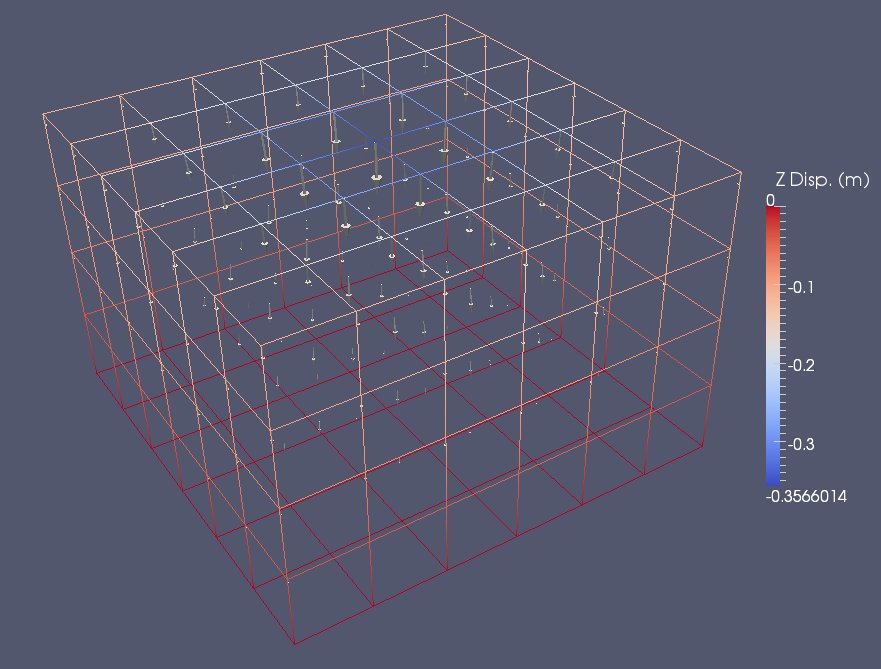
\includegraphics[width=10cm]{tutorials/3dhex8/figs/step18-displ}
\par\end{centering}

\caption{Displacement field for example step18 visualized using ParaView. The
vectors show the displacement field while the colors in the wireframe
correspond to the z-component of the displacement field.\label{fig:step18-displ}}
\end{figure}



\subsubsection{Step19 - Time-Dependent Surface Load}

The \texttt{step19.cfg} file defines a problem that is identical to
example step18, except that we vary the amplitude of the surface load
as a function of time. We use a temporal database (analogous to our
spatial databases for specifying spatial variations) to prescribe
a piecewise linear variation of the amplitude with time as given in
the file \texttt{spatialdb/loadcycle.timedb}. The amplitude begins
at zero, progresses to 1.0, then 1.5, before decreasing in a symmetric
fashion. The temporal database can use variable time steps to prescribe
arbitrary time histories. 

Rather than specify a spatial database for the initial value of the
Neumann boundary condition corresponding to the surface load, we specify
a spatial database for the change in value and the temporal database:
\begin{lyxcode}
{[}pylithapp.timedependent.bc.z\_pos{]}

label~=~face\_zpos

db\_change~=~spatialdata.spatialdb.SimpleDB

db\_change.label~=~Amplitude~of~Neumann~BC~on~+z

db\_change.iohandler.filename~=~spatialdb/tractions\_axial\_pressure.spatialdb

\#~Use~linear~interpolation

db\_change.query\_type~=~linear~\\


th\_change~=~spatialdata.spatialdb.TimeHistory

th\_change.label~=~Time~history~for~Neumann~BC~on~+z

th\_change.filename~=~spatialdb/loadcycle.timedb
\end{lyxcode}
When we have run the simulation, the output VTK files will be contained
in \texttt{examples/3d/hex8/output} (all with a prefix of \texttt{step19}).
Results using ParaView are shown in Figure \ref{fig:step19-stress-t200}.
We also output the solution at user-defined locations, which are given
in the file \texttt{output\_points.txt.} See Section \ref{sec:output:points}
for a discussion of the output parameters. This type of output is
designed for comparison against observations and inversions and output
via HDF5 files (see Section \ref{sub:HDF5/Xdmf-Output}).

\begin{figure}
\begin{centering}
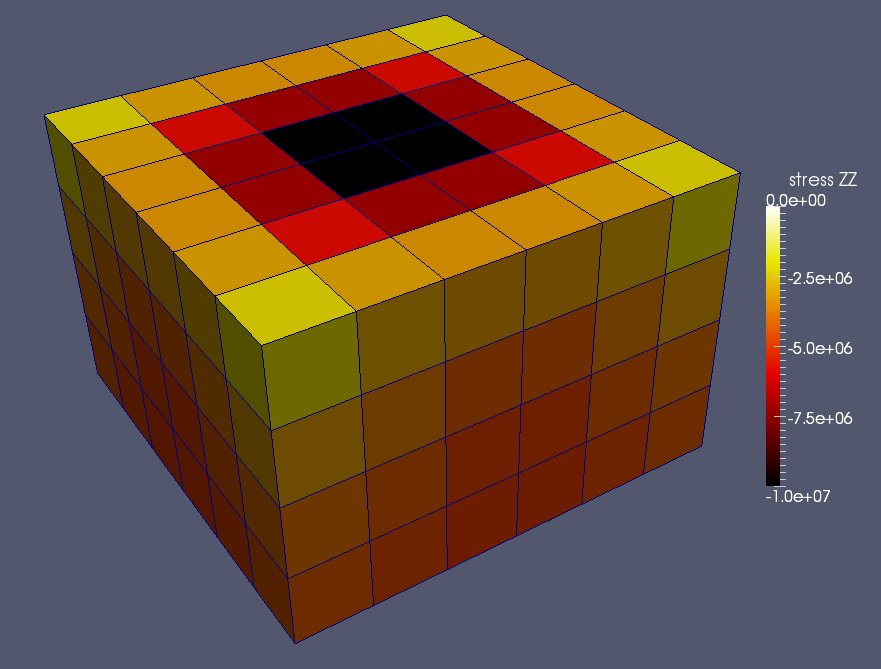
\includegraphics[width=10cm]{tutorials/3dhex8/figs/step19-stress_t200}
\par\end{centering}

\caption{Stress field (zz-component) for example step19 at t = 200 years visualized
using ParaView. The stresses appear as four layers since we have used
\texttt{CellFilterAvg} for material output.\label{fig:step19-stress-t200}}
\end{figure}


\subsection{\label{sec:Tutorial-3d-hex8-dike}Dike Intrusion Example}

PyLith features discussed in this tutorial:
\begin{itemize}
\item Fault opening via prescribed tractions to mimic a dike instrusion
\item Dirichlet boundary conditions
\item Elastic material
\item VTK output
\end{itemize}

\subsubsection{Overview}

This set of examples describes a problem where prescribed tensile
tractions are imposed on a fault to mimic a dike intrusion. The example
is contained in the directory \texttt{examples/3d/hex8}, and the corresponding
\texttt{.cfg} file is \texttt{step20.cfg}. The example may be run
as follows:
\begin{lyxcode}
pylith~step20.cfg
\end{lyxcode}
This will cause PyLith to read the default parameters in \texttt{pylithapp.cfg},
and then override or augment them with the additional parameters in
the \texttt{step20.cfg} file. The \texttt{.cfg} file is extensively
documented, to provide detailed information on the various parameters.


\subsubsection{Step20 - Static Dike Intrusion}

The \texttt{step20.cfg} file defines a problem with spatially varying
tensile normal tractions on the fault surface associated with a fluid
intrusion. The lateral sides and bottom of the domain are fixed using
Dirichlet (roller) boundary conditions. As in the other examples,
we also setup output for the ground surface.

We use the FaultCohesiveDyn object to impose tractions on the fault
surface. We must include a fault constitutive model so we choose static
friction with a coefficient of friction of 0.1. The coefficient of
friction is irrelevant for the center of the fault where we impose
uniform tensile tractions (10 MPa) and the fault opens, but it facilitates
clamping the edges of the fault via compressive normal tractions (-100
MPa). Note that we must set the property \texttt{open\_free\_surface}
to False in order for the tractions to be imposed when the fault is
open; the default behavior for fault opening is a free surface (the
two sides of the fault are completely uncoupled). The most important
fault parameters for prescribing the tensile fault tractions are
\begin{lyxcode}
{[}pylithapp.timedependent.interfaces.fault{]}

open\_free\_surface~=~False~\\


traction\_perturbation~=~pylith.faults.TractPerturbation~\\


{[}pylithapp.timedependent.interfaces.fault.traction\_perturbation{]}

db\_initial~=~spatialdata.spatialdb.SimpleDB

db\_initial.label~=~Initial~fault~tractions

db\_initial.iohandler.filename~=~spatialdb/tractions\_opening.spatialdb

db\_initial.query\_type~=~nearest~
\end{lyxcode}
When we have run the simulation, the output VTK files will be contained
in \texttt{examples/3d/hex8/output} (all with a pvrefix of \texttt{step20}).
Results using ParaView are shown in Figure \vref{fig:step20-disp}.

\begin{figure}
\begin{centering}
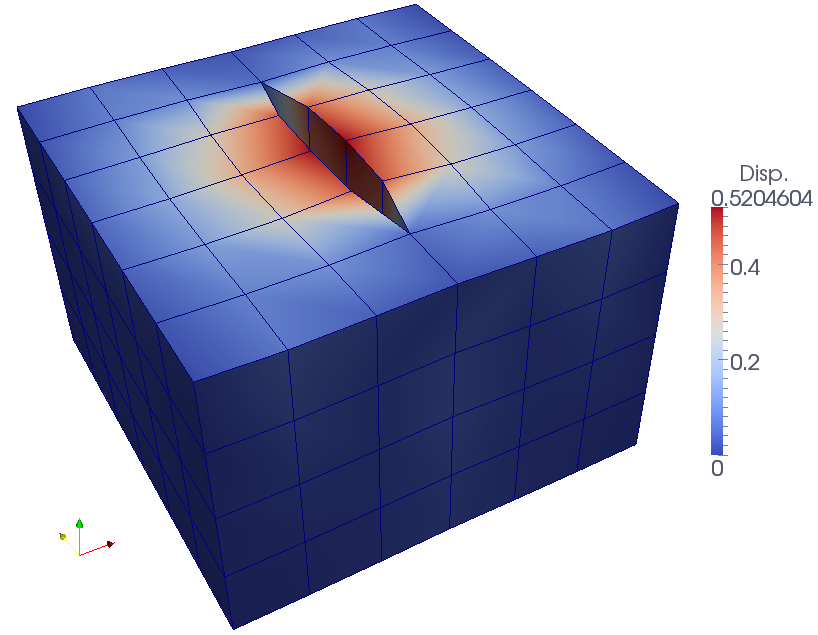
\includegraphics[width=10cm]{tutorials/3dhex8/figs/step20_disp}
\par\end{centering}

\caption{Displacement magnitude for example step20 visualized using ParaView.
\label{fig:step20-disp}}
\end{figure}


\subsection{\label{sec:Tutorial-3d-hex8-greensfns}Green's Functions Generation
Example}

PyLith features discussed in this tutorial:
\begin{itemize}
\item Generation of Green's functions from a fault
\item Kinematic fault impulses
\item Running a different problem type
\item Dirichlet boundary conditions
\item Elastic material
\item HDF5 output
\item Interpolated point output
\end{itemize}

\subsubsection{Overview}

This example describes a problem where we generate a set of Green's
functions that could be used in an inversion. The example is contained
in the directory \texttt{examples/3d/hex8}, and the corresponding
\texttt{.cfg} file is \texttt{step21.cfg}. The example may be run
as follows:
\begin{lyxcode}
pylith~step21.cfg~-{}-problem=pylith.problems.GreensFns
\end{lyxcode}
This will cause PyLith to read the default parameters in \texttt{pylithapp.cfg}
and \texttt{greensfns.cfg}, and then override or augment them with
the additional parameters in the \texttt{step21.cfg} file. The \texttt{.cfg}
files are extensively documented, to provide detailed information
on the various parameters.


\subsubsection{Step21 - Green's Function Generation}

This problem makes use of two \texttt{.cfg} files that are read by
default -- \texttt{pylithapp.cfg} and \texttt{greensfns.cfg}. The
\texttt{greensfns.cfg} file is read automatically because we have
changed the problem type to \texttt{GreensFns} (as opposed to the
default \texttt{TimeDependent} problem type). The facility name then
becomes \texttt{greensfns}, and PyLith will thevrefore search for a
\texttt{.cfg} file matching the name of the facility. The \texttt{greensfns.cfg}
file contains settings that are specific to the \texttt{GreensFns}
problem type:
\begin{lyxcode}
{[}greensfns{]}

fault\_id~=~10



{[}greensfns.interfaces{]}

fault~=~pylith.faults.FaultCohesiveImpulses



{[}greensfns.interfaces.fault{]}

impulse\_dof~=~{[}0,~1{]}

db\_impulse\_amplitude.label~=~Amplitude~of~slip~impulses

db\_impulse\_amplitude.iohandler.filename~=~spatialdb/impulse\_amplitude.spatialdb

db\_impulse\_amplitude.query\_type~=~nearest~
\end{lyxcode}
We specify the \texttt{fault\_id}, which is required by the \texttt{GreensFns}
problem type (it is the same as the ID used when generating the mesh).
We also change the fault type to \texttt{FaultCohesiveImpulses}, which
allows us to apply a single impulse of slip for each impulse with
a nonzero slip value in the corresponding \texttt{spatialdb} file
(\texttt{spatialdb/impulse\_amplitude.spatialdb}). We indicate that
we would like to apply slip impulses in both the left-lateral (\texttt{impulse\_dof}
= 0) and updip (\texttt{impulse\_dof} = 1) directions, and we use
nearest-neighbor interpolation to determine the amount of applied
slip. Note that in the \texttt{spatialdb/impulse\_amplitude.spatialdb}
file we specify negative slip, thus reversing the sense of applied
slip for both slip directions. Note that we also put a margin of zeros
around the edge of the fault, which prevents impulses from being applied
along this boundary.

The \texttt{step21.cfg} file defines the remainder of the parameters
for this problem. The boundary conditions and fault information are
provided as for previous examples. Rather than computing the solution
over the ground surface, we choose to provide output at a set of points.
PyLith provides the ability to interpolate displacements to a specified
set of points, which would generally be necessary when generating
Green's functions:
\begin{lyxcode}
{[}pylithapp.problem.formulation{]}

output~=~{[}domain,points{]}

output.points~=~pylith.meshio.OutputSolnPoints



{[}pylithapp.problem.formulation.output.points{]}

writer~=~pylith.meshio.DataWriterHDF5

writer.filename~=~output/step21-points.h5

reader.filename~=~greensfns\_points.txt

coordsys.space\_dim~=~3

coordsys.units~=~m
\end{lyxcode}
We first define \texttt{OutputSolnPoints} as the output manager for
points output. We use HDF5 output for all of the Green's function
output, as it will generally be more efficient (faster I/O, smaller
file sizes). We must provide a set of points for point output. The
file \texttt{greensfns\_points.txt} contains a set of (x,y,z) coordinates.
We must also provide the spatial dimension of the coordinates as well
as the units used. Note that we do not output any info or data fields
for state variable output, as this would otherwise create a large
amount of output for each applied slip impulse. When we have run the
simulation, the output HDF5 files will be contained in \texttt{examples/3d/hex8/output}
(all with a pvrefix of \texttt{step21}). In Figure \vref{fig:step21-imp-resp}
we show an impulse of left-lateral slip applied on the fault and the
resulting response at the specified set of points. The time corresponds
to the impulse number in multiples of the specified time step size.

\begin{figure}
\begin{centering}
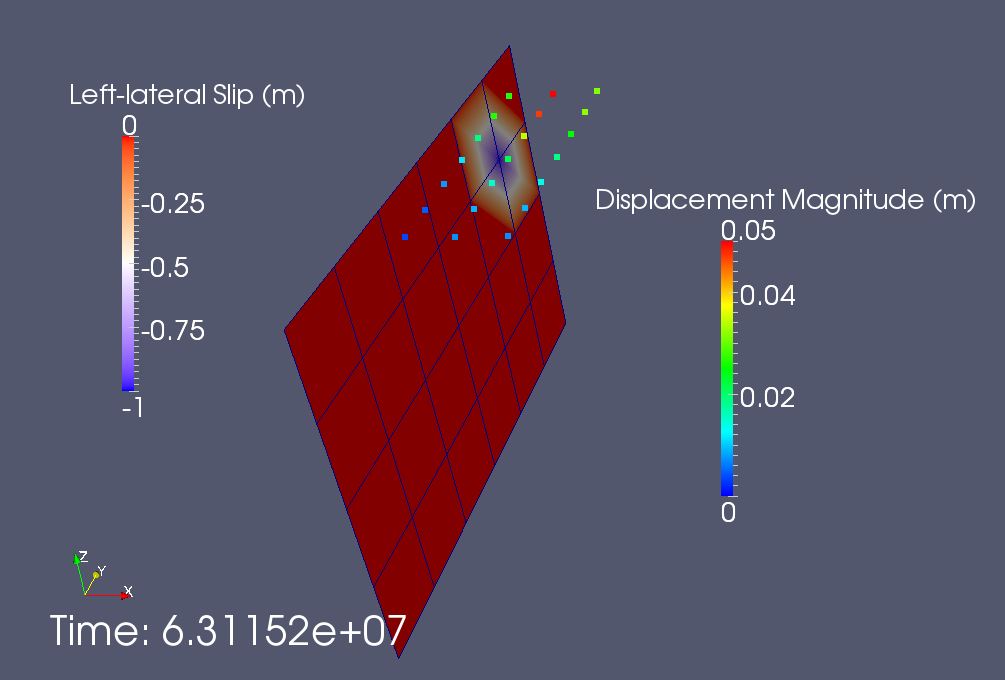
\includegraphics[width=10cm]{tutorials/3dhex8/figs/step21_impulse_resp}
\par\end{centering}

\caption{A slip impulse and the resulting point displacement responses visualized
using ParaView. \label{fig:step21-imp-resp}}
\end{figure}


